% Options for packages loaded elsewhere
\PassOptionsToPackage{unicode}{hyperref}
\PassOptionsToPackage{hyphens}{url}
\PassOptionsToPackage{dvipsnames,svgnames,x11names}{xcolor}
%
\documentclass[
  10pt,
]{article}
\usepackage{amsmath,amssymb}
\usepackage{iftex}
\ifPDFTeX
  \usepackage[T1]{fontenc}
  \usepackage[utf8]{inputenc}
  \usepackage{textcomp} % provide euro and other symbols
\else % if luatex or xetex
  \usepackage{unicode-math} % this also loads fontspec
  \defaultfontfeatures{Scale=MatchLowercase}
  \defaultfontfeatures[\rmfamily]{Ligatures=TeX,Scale=1}
\fi
% lmodern omitted
\ifPDFTeX\else
  % xetex/luatex font selection
  \setmainfont[]{DejaVu Serif}
  \setsansfont[]{DejaVu Sans}
  \setmonofont[]{DejaVu Sans Mono}
  \setmathfont[]{DejaVu Math TeX Gyre}
\fi
% Use upquote if available, for straight quotes in verbatim environments
\IfFileExists{upquote.sty}{\usepackage{upquote}}{}
\IfFileExists{microtype.sty}{% use microtype if available
  \usepackage[]{microtype}
  \UseMicrotypeSet[protrusion]{basicmath} % disable protrusion for tt fonts
}{}
\makeatletter
\@ifundefined{KOMAClassName}{% if non-KOMA class
  \IfFileExists{parskip.sty}{%
    \usepackage{parskip}
  }{% else
    \setlength{\parindent}{0pt}
    \setlength{\parskip}{6pt plus 2pt minus 1pt}}
}{% if KOMA class
  \KOMAoptions{parskip=half}}
\makeatother
\usepackage{xcolor}
\usepackage[margin=2.2cm]{geometry}
\usepackage{longtable,booktabs,array}
\usepackage{calc} % for calculating minipage widths
% Correct order of tables after \paragraph or \subparagraph
\usepackage{etoolbox}
\makeatletter
\patchcmd\longtable{\par}{\if@noskipsec\mbox{}\fi\par}{}{}
\makeatother
% Allow footnotes in longtable head/foot
\IfFileExists{footnotehyper.sty}{\usepackage{footnotehyper}}{\usepackage{footnote}}
\makesavenoteenv{longtable}
\usepackage{graphicx}
\makeatletter
\def\maxwidth{\ifdim\Gin@nat@width>\linewidth\linewidth\else\Gin@nat@width\fi}
\def\maxheight{\ifdim\Gin@nat@height>\textheight\textheight\else\Gin@nat@height\fi}
\makeatother
% Scale images if necessary, so that they will not overflow the page
% margins by default, and it is still possible to overwrite the defaults
% using explicit options in \includegraphics[width, height, ...]{}
\setkeys{Gin}{width=\maxwidth,height=\maxheight,keepaspectratio}
% Set default figure placement to htbp
\makeatletter
\def\fps@figure{htbp}
\makeatother
\setlength{\emergencystretch}{3em} % prevent overfull lines
\providecommand{\tightlist}{%
  \setlength{\itemsep}{0pt}\setlength{\parskip}{0pt}}
\setcounter{secnumdepth}{-\maxdimen} % remove section numbering
\ifLuaTeX
\usepackage[bidi=basic]{babel}
\else
\usepackage[bidi=default]{babel}
\fi
\babelprovide[main,import]{czech}
\ifPDFTeX
\else
\babelfont{rm}[]{DejaVu Serif}
\fi
% get rid of language-specific shorthands (see #6817):
\let\LanguageShortHands\languageshorthands
\def\languageshorthands#1{}
\usepackage{caption}
\captionsetup{labelformat=empty,font=small}
\usepackage{float}
\floatplacement{figure}{!htbp}
\usepackage{needspace}
\usepackage{etoolbox}
\pretocmd{\section}{\Needspace{10\baselineskip}}{}{}
\pretocmd{\subsection}{\Needspace{7\baselineskip}}{}{}
\usepackage{lastpage}
\usepackage{fancyhdr}
\fancypagestyle{plain}{\fancyhf{}\renewcommand{\headrulewidth}{0pt}\fancyfoot[C]{\small\thepage\,/\,\pageref*{LastPage}}}
\pagestyle{plain}
\widowpenalty=10000
\clubpenalty=10000
\renewcommand{\abstractname}{Abstrakt}
\ifLuaTeX
  \usepackage{selnolig}  % disable illegal ligatures
\fi
\IfFileExists{bookmark.sty}{\usepackage{bookmark}}{\usepackage{hyperref}}
\IfFileExists{xurl.sty}{\usepackage{xurl}}{} % add URL line breaks if available
\urlstyle{same}
\hypersetup{
  pdftitle={Různé nástroje, stejný akord: hřeben rezonancí a fáze
prvního řádu u Dirichletových L-funkcí s komplexními charaktery,
sjednocení kruhového tělesa a robustnost hlavní rezonance studie VI -
reprodukovatelná numerická studie VII},
  pdfauthor={David Hess (MAYAN ALFA V1008 LAB v.34.116)},
  pdflang={cs},
  colorlinks=true,
  linkcolor={Maroon},
  filecolor={Maroon},
  citecolor={Blue},
  urlcolor={Blue},
  pdfcreator={LaTeX via pandoc}}

\title{Různé nástroje, stejný akord: hřeben rezonancí a fáze prvního
řádu u Dirichletových L-funkcí s komplexními charaktery, sjednocení
kruhového tělesa a robustnost hlavní rezonance studie VI ---
reprodukovatelná numerická studie VII}
\author{David Hess (MAYAN ALFA V1008 LAB v.34.116)}
\date{23. 11. 2026}

\begin{document}
\hyphenation{ne-roz-hod-nu-to}
\maketitle
\begin{abstract}
Studie VI této řady změřila hřeben rezonancí v rozptylu okénkových
součtů \(\sum g\,x^{i\gamma}\) přes nuly \(\zeta\) a Dirichletových
L-funkcí s reálnými charaktery, ve shodě s dvoubodovými funkcemi
Bogomolného a Keatinga. Zde se měření rozšiřuje na komplexní charaktery
a otázka zní, co závisí na charakteru a co jen na jeho modulu. Každé
pravidlo bylo zapsáno dřív, než byly spočteny nuly, nebo, u pozdějších
doplnění, dřív, než byla veličina vyhodnocena. Na 1 296 658 nově
spočtených nulách 16 Dirichletových L-funkcí modulů 5, 7, 13, 15 a 21
mezi výškami 36 000 a 80 000 (dvanáct s komplexními charaktery a čtyři,
které doplňují rodiny modulů 15 a 21): (1) u dvanácti L-funkcí s
komplexními charaktery závisí hřeben jen na modulu --- průměr \(z^2\)
přes 201 bodů 0,13--0,25 proti dvoubodové funkci bez Eulerových činitelů
\(p \mid q\) a 11,5--49 proti GUE bez aritmetiky, se stejným hřebenem u
všech 18 dvojic L-funkcí téhož modulu; (2) první řád nese fázi
\(\chi(p)\): první Fourierův koeficient \(\{\gamma\ln p/2\pi\}\) se
rovná \(-w\chi(p)\ln p/\sqrt p\) na \(5{,}2\cdot10^{-5}\) v 56
kombinacích těchto L-funkcí a prvočísel a sdružená fáze je vyloučena;
(3) ve sjednocení všech charakterů modulu, což jsou nuly Dedekindovy
zeta funkce tělesa \(\mathbb{Q}(\zeta_q)\) pro \(q = 5, 7, 15, 21\) (až
947 573 nul), zní prvočíslo jen v harmonických, které jsou násobky jeho
řádu modulo \(q\); (4) L-funkce téhož modulu sdílejí prvočísla a křížová
kovariance jejich okénkových součtů se rovná prvočíselné stopě s
relativní fází \(\chi_a\bar\chi_b\); (5) rozptyl počtu nul se nasycuje
na úrovni dané modulem; (6) hlavní rezonance studie VI drží i pro jiné
okno, šest odhadů chyby a plnou kovarianci průběhu, s GUE vzdáleným 12
až 69 chyb podle odhadu chyby.

Tři slepé testy z toho dělají použití: z nul samotných byly správně
určeny modul a charakter, prvočísla dělící modul a řády 16 prvočísel ve
čtyřech kruhových tělesech, v každém testu 16 ze 16. Tři další měření
spojují data s náhodnými maticemi: párová korelace každé L-funkce do tří
středních rozestupů sleduje dvoubodovou funkci Bogomolného a Keatinga
(\(\chi^2\) na koš 0,78--1,86), a ne samotné GUE (6,3--16,5); rozestupy
sjednocení souhlasí se složením nezávislých spekter GUE, jednoho pro
každý charakter, na 0,010 v hustotě, s malým úbytkem nejmenších
rozestupů; a odchylka od GUE slábne s výškou podle předpovědi: mezi
pásmy 36 000--80 000 a 400 000--420 000 klesá její velikost na
\(0{,}719 \pm 0{,}021\) původní hodnoty, předpověď je 0,727. Test počtu
Turingova typu našel dvě dvojice těsných nul, které vyhledávací mřížka
přeskočila; byly doplněny před vyhodnocením. Jediné chybné čtení mimo
testy, řád prvočísla 11 v \(\mathbb{Q}(\zeta_{21})\), vysvětluje
rozlišení pásma: u \(11^5\) slyší sjednocení prvočíslo 161 071 o dvacet
kroků vedle. Všech 18 hypotéz je podpořeno. Tvrzení testovaná v (2)--(4)
jsou věty nebo jejich přímé důsledky; dvoubodová funkce za (1), (5), (6)
a za párovou korelací je domněnka. Přidána jsou data pro komplexní
charaktery s nulovými modely a chybami, nuly, které neexistovaly, když
se psala pravidla, a slepé testy.
\end{abstract}

\hypertarget{uxfavod}{%
\section{1. Úvod}\label{uxfavod}}

Studie VI této řady {[}6{]} změřila rozptyl okénkového součtu
\(\sum_\gamma g\,x^{i\gamma}\) přes nuly \(\zeta\) a našla hřeben
rezonancí u \(x = (T/2\pi)\cdot A/B\), ve shodě s dvoubodovou funkcí
Bogomolného a Keatinga {[}7{]} a daleko od náhodných matic bez
aritmetiky. U osmi Dirichletových L-funkcí s reálnými charaktery
\(\chi_D\) hřeben souhlasil s dvoubodovou funkcí pro Dirichletovy
L-funkce {[}8{]}, která se od funkce pro \(\zeta\) liší jen konečnými
součiny přes prvočísla dělící modul. Otevřené zůstaly dvě otázky: zda
totéž platí pro komplexní charaktery a jak odolná je hlavní rezonance
vůči volbám měření (tvar okna, odhad chyby, korelované body).

U jedné L-funkce \(L(s, \chi)\) v \(t\)-aspektu obsahuje aritmetický
činitel dvoubodové funkce \(|\chi(n)|^2\), takže její předpověď závisí
na modulu \(q\), a ne na hodnotách \(\chi\) {[}8{]}. Jev prvního řádu je
jiný: podle Landauova vzorce pro \(L(s, \chi)\) {[}9, 10{]}
\[\sum_{T_1 < \gamma \le T_2} x^{\rho} = -\frac{T_2 - T_1}{2\pi}\,\chi(x)\Lambda(x) + O(\ln T_2),\]
takže první Fourierův koeficient zlomkových částí
\(\{\gamma\ln p/2\pi\}\) nese fázi \(\chi(p)\) a prohlubeň jejich
hustoty se posouvá z \(0\) do \(\arg\chi(p)/2\pi\). V jazyce
hypotetického spektrálního výkladu (Hilbert--Pólya; Berry a Keating
{[}11{]}) hrají prvočísla roli periodických drah délky \(\ln p\),
explicitní vzorec je stopový vzorec a charakter působí jako fáze
připojená ke každé dráze. Takovou fázi vidí jednotlivé dráhy (první řád)
a ve spárování dráhy se sebou samou se vyruší (druhý řád). Tato studie
měří obě strany tohoto tvrzení na nových nulách.

Čtyři další srovnání používají data, která už existují. Nuly všech
charakterů modulo \(q\) dohromady jsou nuly Dedekindovy zeta funkce
kruhového tělesa \(\mathbb{Q}(\zeta_q)\); v tomto sjednocení se členy
prvního řádu vyruší s výjimkou mocnin prvočísel
\(p^k \equiv 1 \pmod q\), takže nuly mají odrážet, jak se prvočísla v
tělese rozkládají. Je to číselně-teoretická obdoba rozkladu spektra s
diskrétní symetrií na sektory symetrie {[}12, 13{]}. Za druhé, různé
L-funkce téhož modulu sdílejí prvočísla, takže okénkové součty dvou
takových L-funkcí jsou korelované, s relativní fází
\(\chi_a(p)\overline{\chi_b(p)}\), všude tam, kde přispívá málo
prvočísel. Za třetí, rozptyl počtu nul se nasycuje na úrovni dané
prvočísly (Berry {[}14{]}); u \(L(s, \chi)\) má opět záviset jen na
\(q\). Za čtvrté, první nuly všech dvanácti L-funkcí se porovnávají s
LMFDB {[}15{]}.

Dvě další části přidaly datované dodatky dřív, než byla vyhodnocena
data, kterých se týkají. Tři slepé testy se ptají, zda hřeben a první
řád stačí k tomu, aby se z nul samotných poznala L-funkce, prvočísla
dělící její modul a rozklad prvočísel v kruhovém tělese (oddíl 5). Tři
měření spojují data s teorií náhodných matic: párová korelace jedné
L-funkce na krátké vzdálenosti, rozestupy sjednocení proti složení
nezávislých spekter a závislost odchylky od GUE na výšce (oddíl 3.9).

Studie je numerická. Každý testovaný vzorec je buď věta nebo její přímý
důsledek (Landauův vzorec, explicitní vzorec, ortogonalita charakterů),
nebo domněnka s výslovnou předpovědí (dvoubodová funkce Bogomolného a
Keatinga). Nic zde se netýká Riemannovy hypotézy ani existence
hamiltoniánu; měření jsou podmínky, které by každá taková konstrukce
musela splnit.

\hypertarget{data}{%
\section{2. Data}\label{data}}

\textbf{Dvanáct nových L-funkcí (sada hr7).} Primitivní charaktery
modulo \(q = 5\) (řád 4), \(7\) (řády 3 a 6), \(13\) (řád 12), \(15\)
(řád 4, \(p \mid q\): 3, 5) a \(21\) (řád 6, \(p \mid q\): 3, 7), každý
se svým komplexně sdruženým --- Conreyho značení 5.2, 5.3; 7.2, 7.4,
7.3, 7.5; 13.2, 13.7; 15.2, 15.8; 21.5, 21.17. Všechny nuly s
\(36\,000 < \gamma \le T_2\) spočetl PARI/GP 2.17.2 {[}16{]}
(\texttt{lfunzeros}, okna šířky 100, \texttt{divz} 32, úplnost hlídána
proti hladkému počtu \((\theta_\chi(b) - \theta_\chi(a))/\pi\) v každém
okně) na stolním počítači (9 procesů) poté, co byla zapsána pravidla
této studie; výšky \(T_2 = 80\,000\) dosáhlo všech dvanáct (počty a časy
v oddílu 4.1).

\textbf{Čtyři další L-funkce (sada hr7b).} Aby byly úplné rodiny všech
charakterů modulo 15 a modulo 21, byly v témž pásmu týmž skriptem po
hlavním běhu spočteny nuly \(L(s, \chi_{-15})\) (15.14),
\(L(s, \chi_{21})\) (21.20) a druhého komplexního páru řádu 6 modulo 21
(21.2, 21.11) (dodatek 5 k pravidlům): 82 726, 85 082, 85 083 a 85 082
nul po opravě z oddílu 4.10. Spolu s \(\zeta\), \(\chi_{-3}\),
\(\chi_5\), \(\chi_{-7}\) ze studie VI a se sadou hr7 to dává všech 8
charakterů modulo 15 a všech 12 modulo 21; každý neprimitivní charakter
zastupuje primitivní charakter, který ho indukuje. Sady hr7 a hr7b
dohromady tvoří 16 L-funkcí této studie s 1 296 658 nulami.

\textbf{Druhé pásmo (sada hr7c).} Pro srovnání dvou výšek (oddíl 3.9)
byly nuly čtyř L-funkcí sady hr7b s \(400\,000 < \gamma \le 420\,000\)
spočteny týmž skriptem 22. listopadu 2026 poté, co byla zapsána pravidla
tohoto srovnání a jeho vyhodnocovací skript: 178 844 nul, spočtených na
témž stolním počítači od 20:03 do 23:32 UTC (první a poslední okno).

\textbf{Referenční data z dřívějších studií.} Nuly \(L(s, \chi_5)\),
\(L(s, \chi_{-7})\), \(L(s, \chi_{13})\) v témž pásmu (studie VI
{[}6{]}); nuly \(\zeta\) v témž pásmu z Plattových tabulek {[}17{]} v
LMFDB {[}15{]} (shoda s Odlyzkovým souborem zeros6 {[}18{]} na
\(3\cdot10^{-9}\)); a pro část o robustnosti dvě pásma Plattových nul u
\(t \approx 10^8\) (P8) a \(t \approx 3\cdot10^{10}\) (P3e10) použitá ve
studii VI.

\textbf{Kontroly.} Čtyřicet náhodných nul každé L-funkce vyčísleno v
mpmath přes Hurwitzovu zeta funkci; prvních 25 nul každé z dvanácti
L-funkcí porovnáno s LMFDB (největší rozdíl \(3{,}6\cdot10^{-15}\));
nuly \(L(s, \chi)\) pod reálnou osou se shodují s nulami
\(L(s, \bar\chi)\) nad ní.

\hypertarget{metody}{%
\section{3. Metody}\label{metody}}

\hypertarget{hux159eben-jednuxe9-l-funkce}{%
\subsection{3.1 Hřeben jedné
L-funkce}\label{hux159eben-jednuxe9-l-funkce}}

Jako ve studii VI {[}6{]}: Gaussova okna šířky \(H = 20\) se středy
\(T_0\) po \(H\), \(\ln x = \ln(qT_0/2\pi) + \delta\) s
\(\delta \in [-2{,}5; 2{,}5]\) po krocích 0,025,
\(V(\delta) = \langle|S - \langle S\rangle|^2\rangle/\langle N_2\rangle\),
chyba = větší z \(V/\sqrt M\) (\(M\) nezávislých oken po \(6H\)) a
rozptylu přes deset podpásem. Předpověď \(V_{\mathrm{BK},q}\):
dvoubodová funkce \(\zeta\) bez Eulerových činitelů \(p \mid q\) a s
\(L = \ln(qT/2\pi)\) {[}8{]}, spočtená kódem studie VI beze změny
(shodná se zveřejněnými předpověďmi pro \(q = 5, 7, 13\)). Nulové
předpovědi: táž funkce bez vynětí činitelů („naivní \(\zeta\)``) a GUE
bez aritmetiky.

\hypertarget{stejnuxfd-modul-stejnuxfd-hux159eben-bez-teorie}{%
\subsection{3.2 Stejný modul, stejný hřeben (bez
teorie)}\label{stejnuxfd-modul-stejnuxfd-hux159eben-bez-teorie}}

Pro dvě L-funkce \(a\), \(b\) téhož modulu
\(Q_{ab} = \langle (V_a - V_b)^2/(e_a^2 + e_b^2)\rangle_\delta\).
Kontrolní dvojice různých modulů, kde teorie předpovídá rozdíl
(\(Q_{ab} \approx 15\)--20), ukazují, že test rozdíl vidět umí.

\hypertarget{fuxe1ze-prvnuxedho-ux159uxe1du}{%
\subsection{3.3 Fáze prvního
řádu}\label{fuxe1ze-prvnuxedho-ux159uxe1du}}

Pro každou L-funkci a prvočíslo \(p \nmid q\), \(p \le 13\):
\(c = \langle e^{2\pi i u}\rangle\) s \(u = \{\gamma\ln p/2\pi\}\),
předpověď \(c = -w\,\chi(p)\ln p/\sqrt p\), \(w = (T_2 - T_1)/2\pi N\);
histogram \(u\) proti hustotě
\(1 - 2w\sum_k (\ln p/p^{k/2})\,\mathrm{Re}(\chi(p)^k e^{-2\pi i k u})\)
a proti sdružené fázi.

\hypertarget{sjednocenuxed-kruhovuxe9ho-tux11blesa}{%
\subsection{3.4 Sjednocení kruhového
tělesa}\label{sjednocenuxed-kruhovuxe9ho-tux11blesa}}

\(U_5 = \{\zeta, \chi_5, \chi, \bar\chi\}\) a
\(U_7 = \{\zeta, \chi_{-7}\), dva páry řádu 3 a 6\(\}\):
\(c_k(p) = -w_U\,\varphi(q)\,[p^k \equiv 1 \bmod q]\,\ln p/p^{k/2}\) pro
\(x = p^k \le 200\); histogramy pro \(p = 2, 3\) proti předpovědi s
interferencí a proti alternativě bez interference.

\hypertarget{sduxedlenuxe9-druxe1hy-kux159uxedux17eovuxe1-kovariance}{%
\subsection{3.5 Sdílené dráhy: křížová
kovariance}\label{sduxedlenuxe9-druxe1hy-kux159uxedux17eovuxe1-kovariance}}

\(C_{ab}(x) = \langle (S_a - \langle S_a\rangle)\overline{(S_b - \langle S_b\rangle)}\rangle/\sqrt{N_{2,a}N_{2,b}}\)
v \(\ln x \in \{3,\penalty300 4,\penalty300 5,\penalty300 6\}\) proti prvočíselné stopě
\((H^2/2\pi)\sum_n \chi_a(n)\overline{\chi_b(n)}\Lambda(n)^2 n^{-1}e^{-H^2\ln^2(n/x)}/\sqrt{N_{2,a}N_{2,b}}\).

\hypertarget{nasycenuxed-rozptylu-poux10dtu}{%
\subsection{3.6 Nasycení rozptylu
počtu}\label{nasycenuxed-rozptylu-poux10dtu}}

\(\Sigma^2(\ell)\) rozvinutých nul (\(\theta_\chi(\gamma)/\pi\)),
intervaly začínající každých 0,37, \(\ell \in [0{,}1; 200]\), chyba z
deseti podpásem; předpověď z dvoubodové funkce Bogomolného a Keatinga
bez činitelů \(p \mid q\) (ověřena proti kódu studie VI na
\(5\cdot10^{-5}\)); pro srovnání Berryho diagonální vzorec {[}14{]}.

\hypertarget{robustnost-hlavnuxed-rezonance-nuly-zeta}{%
\subsection{\texorpdfstring{3.7 Robustnost hlavní rezonance (nuly
\(\zeta\))}{3.7 Robustnost hlavní rezonance (nuly \textbackslash zeta)}}\label{robustnost-hlavnuxed-rezonance-nuly-zeta}}

Hannovo okno \(\cos^2(\pi t/2a)\), \(a = 3H\), s předpovědí přepočtenou
pro jeho autokorelaci (ověřeno proti sítu v diagonálním režimu na
\(8\cdot10^{-7}\)); šest odhadů chyby v \(\tau = 1\) (5, 10, 20, 40
podpásem, \(V/\sqrt M\), blokový jackknife); plná kovariance průběhu o
201 bodech s Hotellingovou opravou, efektivní počet nezávislých bodů a
globální \(p\)-hodnota pro největší odchylku. Táž analýza s Hannovým
oknem pro dvanáct L-funkcí.

\hypertarget{pravidla-zapsanuxe1-pux159edem}{%
\subsection{3.8 Pravidla zapsaná
předem}\label{pravidla-zapsanuxe1-pux159edem}}

Pravidla této studie byla zapsána 20. listopadu 2026 v 07:58 UTC, dřív
než byly spočteny nuly sady hr7 (první okno bylo zapsáno v 08:03 UTC).
Následovaly tři datované dodatky, všechny dřív, než byla data přenesena
ze stolního počítače: otisky vyhodnocovacích skriptů po generálce na
zkušební L-funkci (09:15 UTC), pět dalších srovnání navržených ještě bez
pohledu na data (15:14 UTC) a dvě opravy nalezené na zkušebních datech
--- rozptyl počtu se porovnává s plnou dvoubodovou funkcí místo Berryho
diagonálního vzorce a sjednocení kruhového tělesa se posuzuje jen pro
\(x \le 200\), kde je chybový člen Landauova vzorce malý (15:51 UTC). Co
bylo z pásma spočteno před pravidly (jen měření času, žádné statistiky),
je v nich uvedeno.

\hypertarget{srovnuxe1nuxed-s-nuxe1hodnuxfdmi-maticemi-dodatky-9-a-10}{%
\subsection{3.9 Srovnání s náhodnými maticemi (dodatky 9 a
10)}\label{srovnuxe1nuxed-s-nuxe1hodnuxfdmi-maticemi-dodatky-9-a-10}}

O nulách jedné L-funkce vysoko na kritické přímce se má za to, že
lokálně sledují statistiku vlastních čísel velkých náhodných unitárních
matic (GUE): Montgomery {[}22{]} pro párovou korelaci \(\zeta\),
numerika Odlyzka {[}23{]} a Rudnick se Sarnakem {[}24{]} pro hlavní
L-funkce v omezeném rozsahu. V konečné výšce existují aritmetické
opravy. Pro \(\zeta\) plynou z dvoubodové funkce Bogomolného a Keatinga
{[}7{]} a s daty je porovnali Bogomolny, Bohigas, Leboeuf a Monastra
{[}25{]}, kteří ukázali, že v hlavním řádu se nuly u výšky \(T\) chovají
jako vlastní čísla unitárních matic konečné efektivní velikosti. Pro
Dirichletovy L-funkce obsahuje dvoubodová funkce z {[}8{]} opravu téhož
druhu bez Eulerových činitelů prvočísel dělících \(q\); numerické
srovnání v {[}8{]} není. S tímto obrazem spojují naše data tři měření.
Jejich pravidla byla zapsána 22. listopadu 2026, poté co bylo
vyhodnoceno patnáct testů popsaných výše, ale dřív, než byla kterákoli z
těchto statistik spočtena.

\begin{enumerate}
\def\labelenumi{(\roman{enumi})}
\item
  \emph{Párová korelace na krátké vzdálenosti.} S rozvinutím
  \(w = (\gamma/2\pi)(\ln(q\gamma/2\pi) - 1)\) se hustota \(R_2(d)\)
  dvojic v rozvinuté vzdálenosti \(0 < d \le 3\) měří v 60 koších šířky
  0,05 s chybami z deseti bloků a porovnává s tvarem GUE
  \(1 - (\sin\pi d/\pi d)^2\) a s dvoubodovou funkcí z {[}8{]},
  zprůměrovanou přes každý koš a přes pásmo. Mez: \(\chi^2\) na koš
  nejvýš 2,0 proti {[}8{]} u aspoň 14 ze 16 L-funkcí, přičemž GUE je
  aspoň třikrát horší a aspoň 4.
\item
  \emph{Sjednocení jako složení.} Kdyby sektory sjednocení (L-funkce
  charakterů modulo \(q\)) byly statisticky nezávislá spektra GUE s
  podíly hustot \(f_i\), byla by pravděpodobnost, že úsek délky \(s\)
  středních rozestupů sjednocení je prázdný,
  \(E_S(s) = \prod_i E_\mathrm{GUE}(f_i s)\) a hustota rozestupů
  \(p_S = E_S''\) --- pravidlo skládání Rosenzweiga a Portera {[}27{]} a
  Berryho a Robnika {[}28{]}. Že jsou nuly různých L-funkcí statisticky
  nezávislé, takže se nuly součinu chovají jako složení nekorelovaných
  souborů GUE, zdůvodnili Bogomolny a Leboeuf {[}30{]} za předpokladu
  Hardyho--Littlewoodovy domněnky. \(E_\mathrm{GUE}\) je Fredholmův
  determinant sinového jádra, vyčíslený Gaussovou--Legendreovou
  kvadraturou {[}26{]}. Mez, pro všechna čtyři sjednocení: největší
  \(|p - p_S|\) přes 40 košů šířky 0,1 nejvýš 0,015; první koš aspoň o
  0,03 pod Poissonovou hodnotou; jedno spektrum GUE vedle aspoň o 0,2 v
  některém koši.
\item
  \emph{Výška.} Párová korelace z (i) se měří znovu u čtyř L-funkcí sady
  hr7b ve druhém pásmu, \(400\,000 < \gamma \le 420\,000\), jehož nuly
  byly spočteny až po zapsání pravidel. Tam {[}8{]} předpovídá menší
  odchylku od GUE. Měřenou odchylku shrnuje amplituda \(A\) rozdílu
  \(R_2 - R_2^\mathrm{GUE}\) ve tvaru předpovědi
  \(R_2^\mathrm{BK} - R_2^\mathrm{GUE}\) (vážená chybami z bloků) a její
  velikost
  \(V = A\cdot\mathrm{rms}(R_2^\mathrm{BK} - R_2^\mathrm{GUE})\),
  sdruženě přes čtyři L-funkce. Meze: \(\chi^2\) na koš nejvýš 2,0 v
  horním pásmu u aspoň tří ze čtyř; sdružené \(|A - 1|\) do tří chyb;
  sdružená velikost v horním pásmu menší aspoň o tři chyby; poměr
  velikostí do tří chyb od předpovězeného poměru.
\end{enumerate}

Typ symetrie rodiny ve smyslu Katze a Sarnaka {[}29{]} --- unitární pro
všechny charaktery modulu, symplektický pro kvadratické charaktery
studií III a V --- se týká nízko ležících nul přes rodinu. Zde se
netestuje: všechny nuly této studie leží vysoko na kritické přímce.

\hypertarget{laboratoux159-a-pouux17eituxed-asistenta-s-umux11blou-inteligencuxed}{%
\subsection{3.10 Laboratoř a použití asistenta s umělou
inteligencí}\label{laboratoux159-a-pouux17eituxed-asistenta-s-umux11blou-inteligencuxed}}

\textbf{Laboratoř.} Měření vznikala v laboratoři uvedené v řádku autora
(vývojový nástroj autora; není součástí publikace). Každá hypotéza je v
ní zapsána se svým pravidlem, nulovým modelem a verdiktem a list této
studie přepočítává hlavní veličiny z uložených počtů a porovnává je s
výsledky skriptů. Laboratoř je kontrolou evidence, ne zdrojem čísel:
každé číslo tohoto článku je v souborech výsledků v repozitáři.

\textbf{Použití asistenta s umělou inteligencí.} Práce vznikala v
dialogu autora s asistentem s umělou inteligencí (Claude, Anthropic).
Autor určil otázky a rozsah, rozhodl, co se bude měřit a co budou
pravidla žádat, spustil výpočty nul na svém počítači a schválil každý
krok i tento text. Asistent psal a spouštěl skripty, hledal v
literatuře, připravoval znění pravidel a připravil text článku anglicky
i česky. Žádné číslo v článku nepochází z jazykového modelu: každé číslo
spočetl skript z repozitáře (PARI/GP, mpmath, NumPy, SciPy,
python-flint) z dat oddílu 2 a je uloženo v souborech výsledků;
vyhodnocovací skripty dostaly otisk (SHA-256) dřív, než byla otevřena
data, která vyhodnocují, a hlavní čísla přepočítává nezávislý kód. Chyby
nalezené cestou --- mezi nimi dvě přeskočené dvojice nul z oddílu 4.10
--- jsou zapsány v datovaných dodatcích a nebyly odstraněny. Za obsah
odpovídá autor.

\hypertarget{vuxfdsledky}{%
\section{4. Výsledky}\label{vuxfdsledky}}

\hypertarget{data-1}{%
\subsection{4.1 Data}\label{data-1}}

Dvanáct L-funkcí má po 75 032 až 85 082 nulách v
\(36\,000 < \gamma \le 80\,000\), celkem 958 685; všech 440 oken každé
L-funkce je na místě se shodnými otisky SHA-256, nuly rostou a přes celé
pásmo se počty liší od hladkého počtu nejvýš o 1,1. Čtyřicet náhodných
nul každé L-funkce dává v mpmath
\(|L(\tfrac12 + i\gamma, \chi)| \le 1{,}3\cdot10^{-9}\). Výpočet běžel
na stolním počítači od 20. listopadu 08:03 UTC do 23:13 UTC; devět oken
přerušených z klávesnice v terminálu bylo znovu spočteno na témž
počítači týmž příkazem 21. listopadu (00:41--00:43 UTC) a shodují se bit
po bitu s nezávislým přepočtem v cloudu. Když byl týž příkaz spuštěn
znovu, stolní počítač spočetl podruhé také 4 397 z 5 280 oken (21.
listopadu, 00:44--18:23 UTC); všechna jsou bit po bitu shodná s prvním
výpočtem.

\hypertarget{jeden-akord-pro-kaux17eduxfd-nuxe1stroj}{%
\subsection{4.2 Jeden akord pro každý
nástroj}\label{jeden-akord-pro-kaux17eduxfd-nuxe1stroj}}

U všech dvanácti L-funkcí hřeben souhlasí s předpovědí
\(V_{\mathrm{BK},q}\): \(Q = 0{,}13\)--\(0{,}25\) na 201 bodech (2 183
oken, \(M = 364\)), největší \(|z| = 1{,}66\) (obr. 1). GUE bez
aritmetiky dává na týchž chybách \(Q = 11{,}5\)--\(49\), naivní
předpověď \(\zeta\) (činitele \(p \mid q\) nevyňaty)
\(Q = 3{,}3\)--\(64\). Pro \(q = 13\) naivní předpověď odlišit nelze
(\(Q = 0{,}78\)); pravidla předem uváděla, že tam má test malou sílu
(čekané \(Q = 0{,}6\)), protože první zub ovlivněný \(p = 13\) leží mimo
měřený rozsah. Výška zubu u poměru \(A/B = 2\) sleduje modul:

{\small\begin{longtable}[]{@{}llll@{}}
\toprule\noalign{}
\(q\) & vyňatá prvočísla & měřeno (každá L-funkce) & předpověď \\
\midrule\noalign{}
\endhead
\bottomrule\noalign{}
\endlastfoot
5 & 5 & 3,78; 3,87 (\(\pm 0{,}20\)) & 3,81 \\ \addlinespace[2pt]
7 & 7 & 3,30--3,33 (\(\pm 0{,}17\)) & 3,33 \\ \addlinespace[2pt]
13 & 13 & 2,90; 2,91 (\(\pm 0{,}15\)) & 2,87 \\ \addlinespace[2pt]
15 & 3, 5 & 7,15; 7,11 (\(\pm 0{,}37\)) & 7,15 \\ \addlinespace[2pt]
21 & 3, 7 & 6,23; 6,11 (\(\pm 0{,}33; \pm 0{,}32\)) & 6,16 \\ \addlinespace[2pt]
\end{longtable}}

Bez jakékoli teorie má 18 dvojic L-funkcí téhož modulu (včetně reálných
charakterů studie VI) stejný hřeben, \(Q_{ab} = 0{,}13\)--\(0{,}29\),
kdežto kontrolní dvojice různých modulů se liší,
\(Q_{ab} = 15{,}3\)--\(20{,}1\).

Hodnoty \(Q \approx 0{,}15\) místo \(\approx 1\) znamenají, že odhad
chyby hřebene je opatrný asi 2,5krát. Totéž bylo vidět ve studii VI a na
zkušební L-funkci \(q = 11\); odstup od nulových předpovědí to
nezmenšuje, protože se posuzují na týchž chybách.

\begin{figure}
\centering
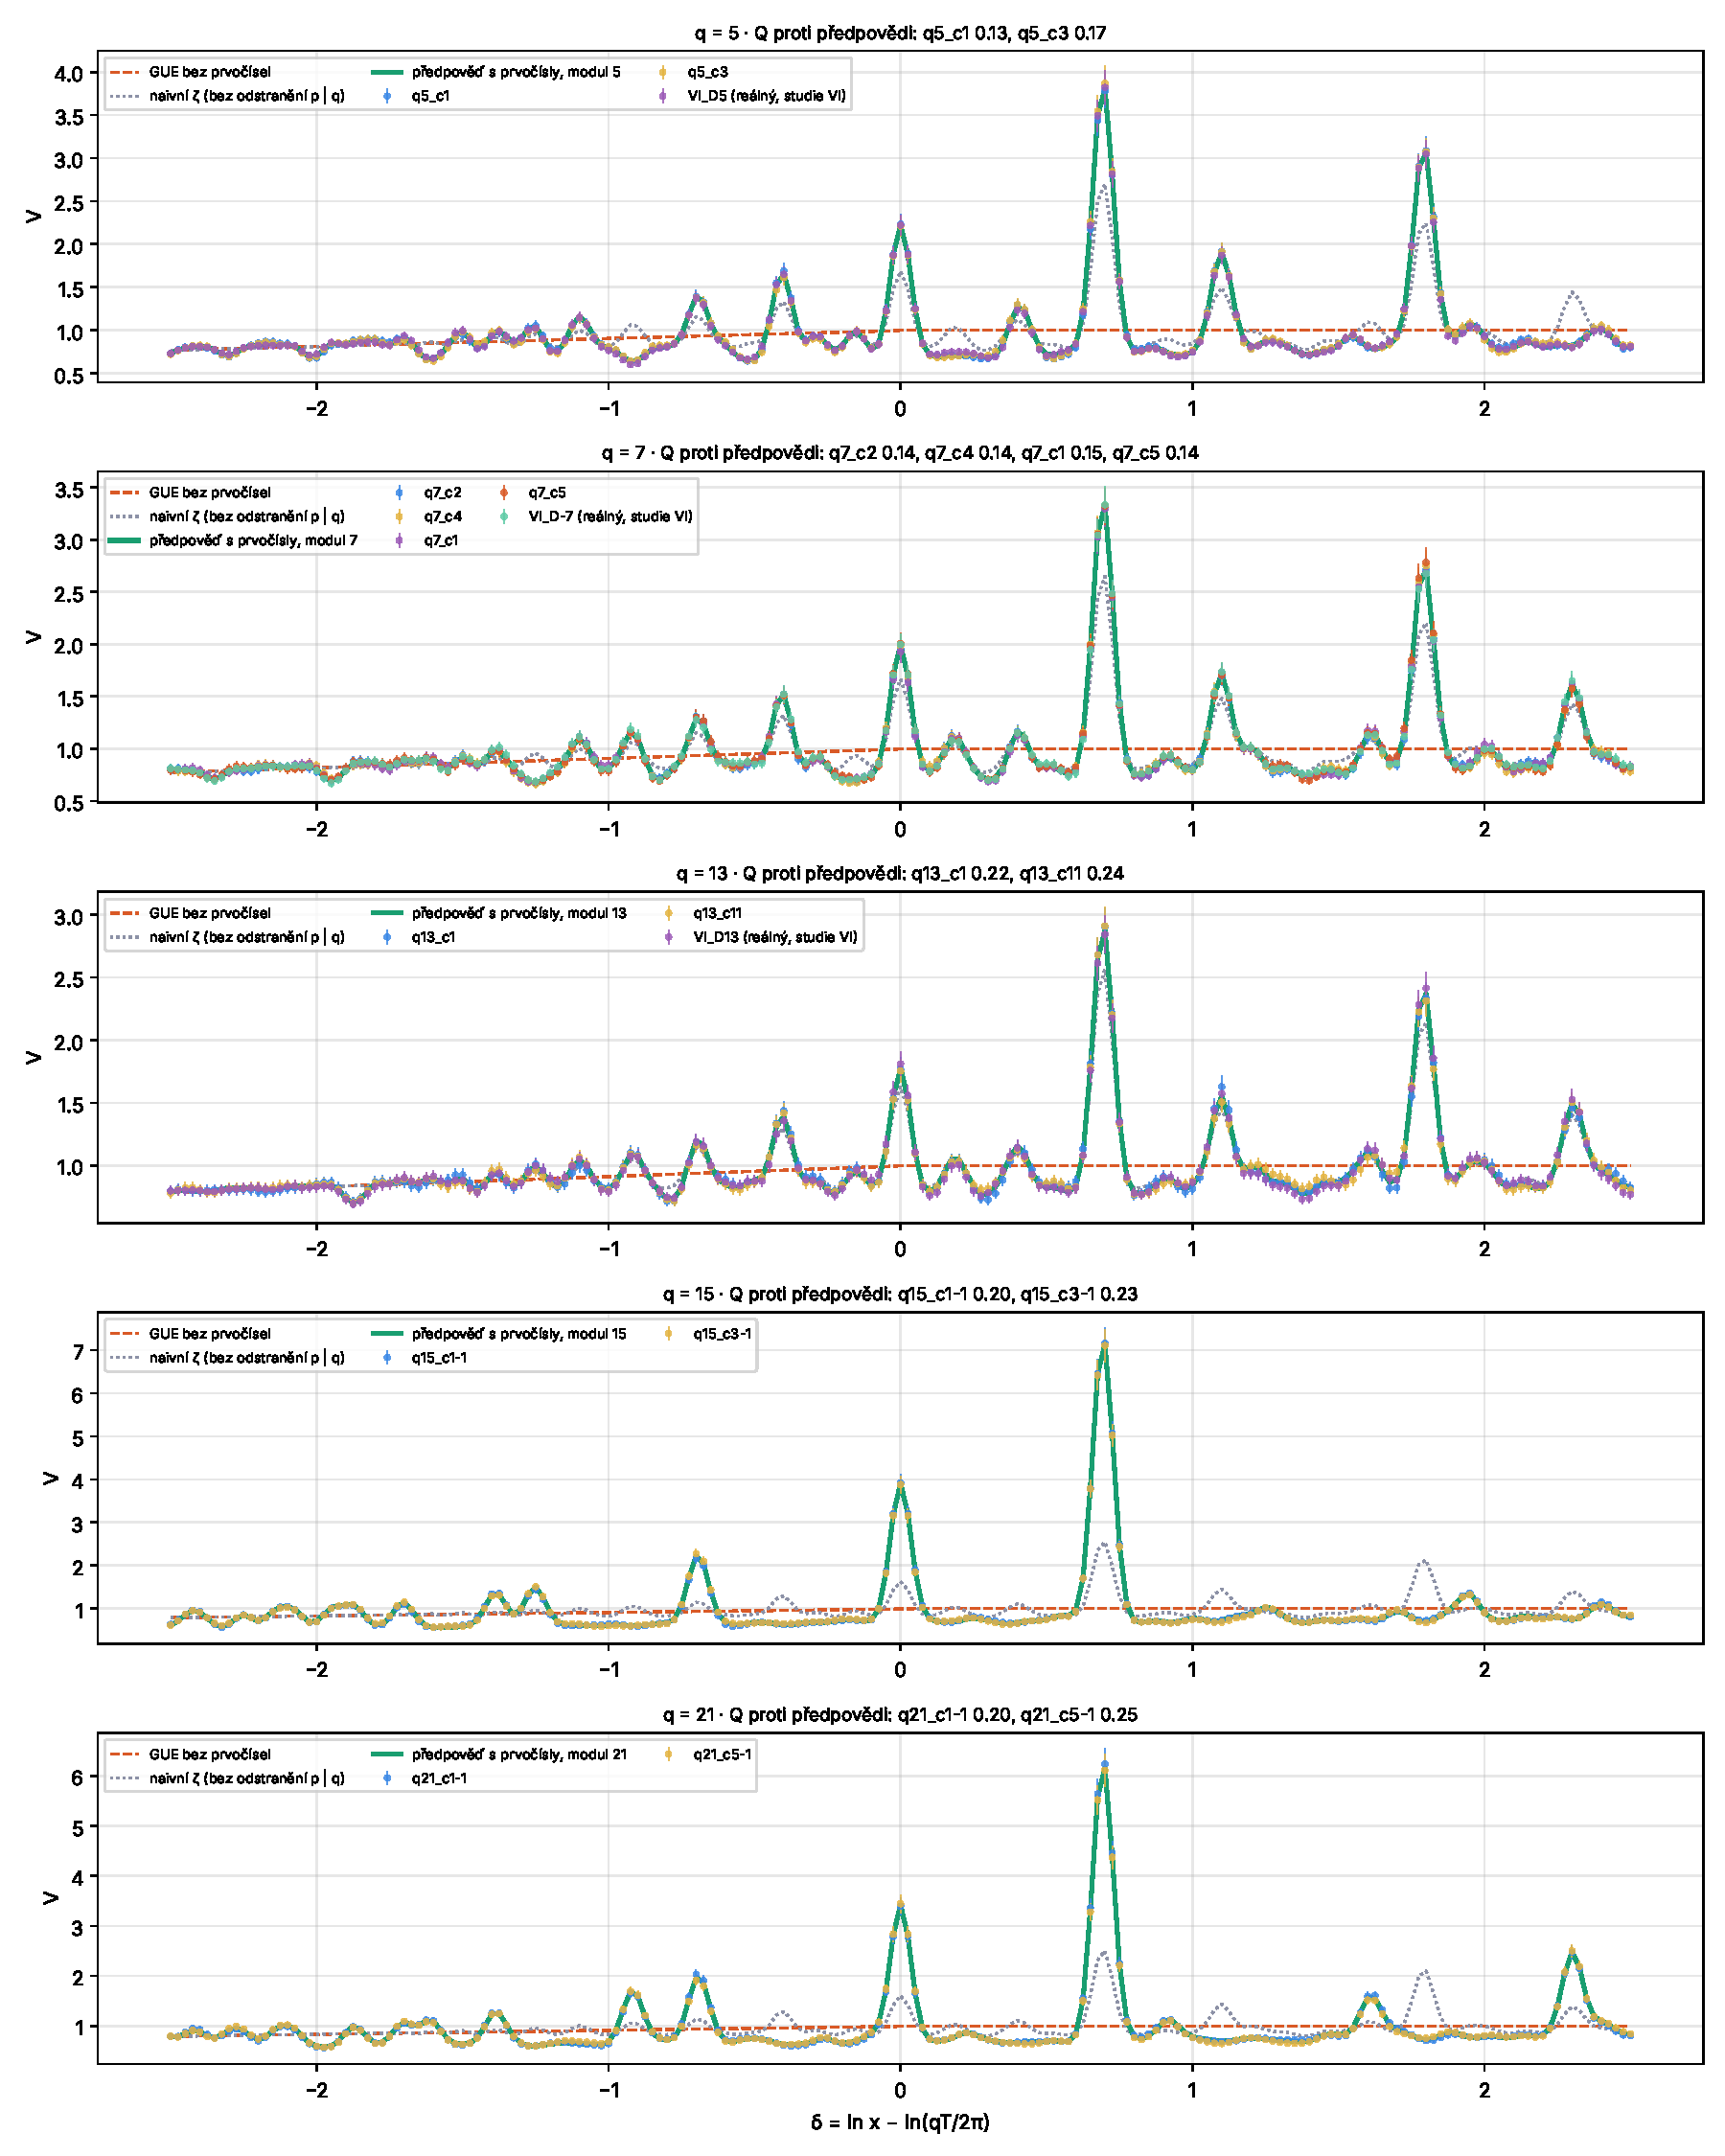
\includegraphics[width=1\textwidth,height=\textheight]{../../figures/01_comb_cz.pdf}
\caption{Obrázek 1. Hřeben rezonancí podle modulu: \(V(\delta)\)
dvanácti L-funkcí sady hr7 a reálných charakterů studie VI (\(\pm 1\)
chyba, výšky 36 000--80 000, \(H = 20\), 201 bodů) proti dvoubodové
funkci bez Eulerových činitelů \(p \mid q\) (plná čára), naivní
předpovědi \(\zeta\) (tečkovaně) a GUE bez aritmetiky (čárkovaně).}
\end{figure}

\hypertarget{melodie-nese-fuxe1zi}{%
\subsection{4.3 Melodie nese fázi}\label{melodie-nese-fuxe1zi}}

U 56 kombinací L-funkce a prvočísla \(p \le 13\), \(p \nmid q\),
souhlasí první Fourierův koeficient \(\{\gamma\ln p/2\pi\}\) s
\(-w\,\chi(p)\ln p/\sqrt p\) na \(5{,}2\cdot10^{-5}\) (obr. 2);
histogramy souhlasí s hustotou sestavenou z \(\chi(p)\) (nejmenší
\(p = 0{,}13\)) a u všech 46 kombinací s komplexním \(\chi(p)\) je
sdružená fáze zamítnuta (\(p \le 7\cdot10^{-154}\)). Prohlubeň hustoty
se posouvá do \(\arg\chi(p)/2\pi\), jak říká Landauův vzorec. Hodnoty
\(\chi^2\) histogramů jsou většinou menší než jejich počet stupňů
volnosti (\(p\) mezi 0,75 a 1): zlomkové části jsou rozloženy
rovnoměrněji, než by byly nezávislé body, což je důsledek tuhosti nul.

Okénkové součty souhlasí se sítem přes mocniny prvočísel na
\(1{,}4\cdot10^{-11}\) (960 bodů; ostré okno až \(6{,}2\cdot10^{-2}\)) a
v diagonálním režimu souhlasí data s prvočíselným součtem na
\(|z| \le 0{,}06\). Nezávislá druhá implementace hřebene a koeficientů
reprodukuje první na \(5{,}9\cdot10^{-12}\) a \(1{,}1\cdot10^{-12}\).

\begin{figure}
\centering
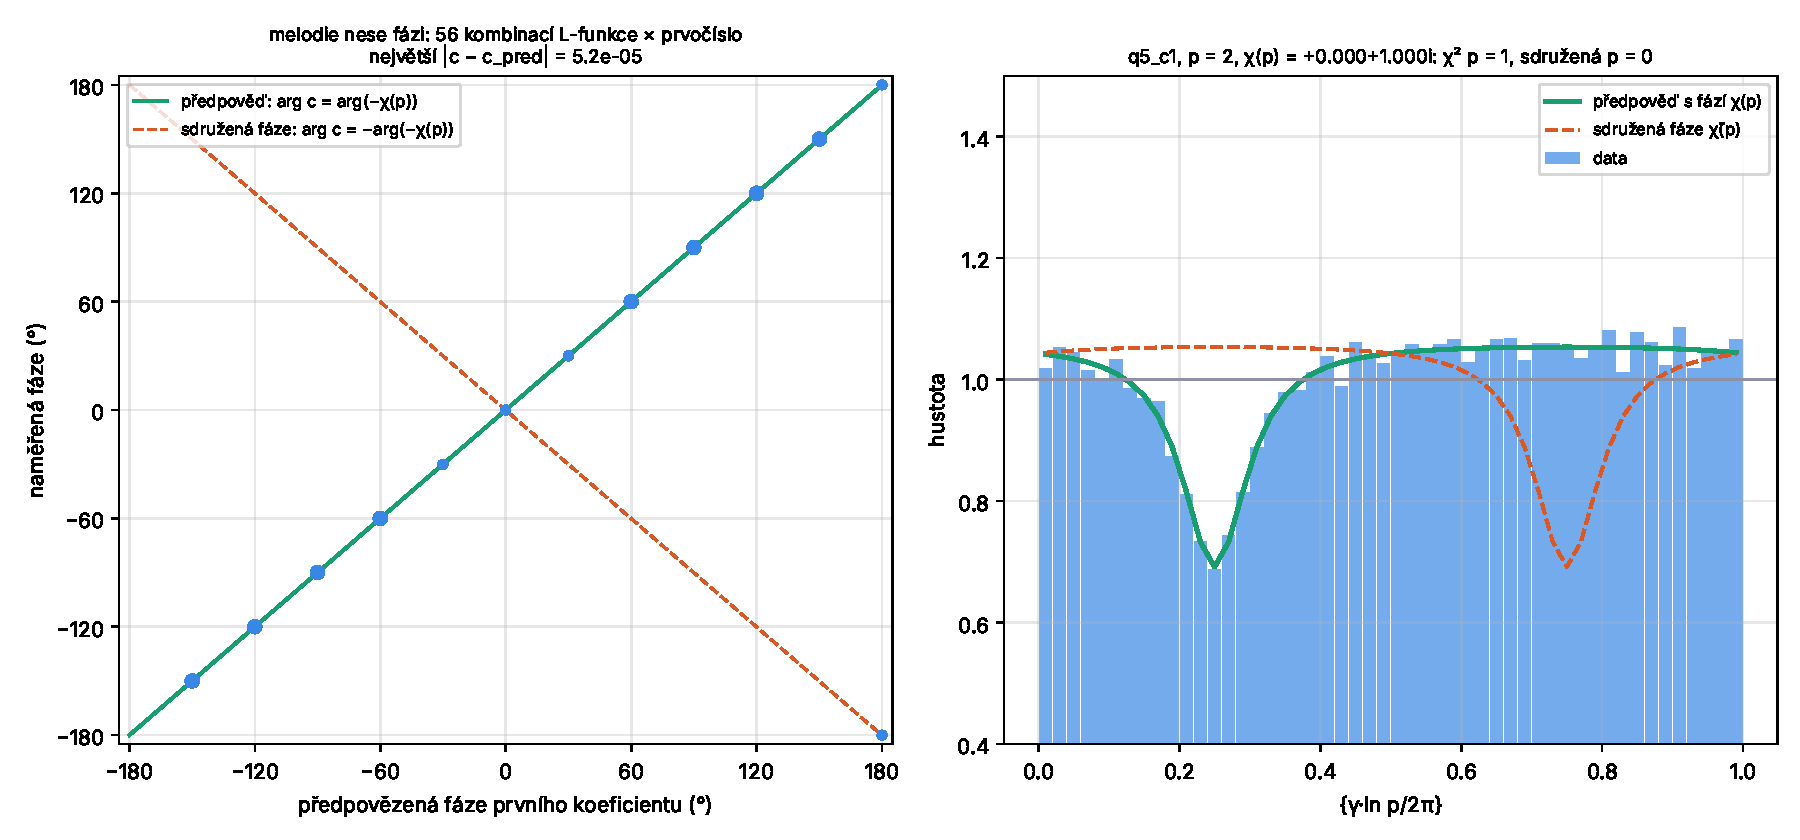
\includegraphics[width=1\textwidth,height=\textheight]{../../figures/02_phase_cz.pdf}
\caption{Obrázek 2. Fáze prvního řádu. Vlevo: naměřená proti
předpovězené fázi prvního Fourierova koeficientu
\(\{\gamma\ln p/2\pi\}\) pro 56 kombinací L-funkce a prvočísla; sdružená
fáze by ležela na klesající přímce. Vpravo: příklad histogramu (5.2,
\(p = 2\), \(\chi(2) = i\)) s hustotou sestavenou z \(\chi(p)\) a ze
sdružené hodnoty.}
\end{figure}

\hypertarget{celuxfd-orchestr-sjednocenuxed-kruhovuxe9ho-tux11blesa}{%
\subsection{4.4 Celý orchestr: sjednocení kruhového
tělesa}\label{celuxfd-orchestr-sjednocenuxed-kruhovuxe9ho-tux11blesa}}

Ve sjednocení všech charakterů modulo 5 (\(N_U = 288\,861\) nul) a
modulo 7 (\(N_U = 450\,707\)) koeficienty prvního řádu vymizí s výjimkou
\(p^k \equiv 1 \pmod q\), jak říká předpověď: největší
\(|c - c_{\mathrm{pred}}|\) pro \(x = p^k \le 200\) je
\(7{,}2\cdot10^{-5}\) a \(4{,}8\cdot10^{-5}\); histogramy pro
\(p = 2, 3\) souhlasí s předpovědí s interferencí
(\(p = 0{,}999; 0{,}895\) a \(0{,}973; 0{,}968\)) a zamítají alternativu
bez interference (\(p \approx 0\)). Čteno jen z dat, řád \(\hat f(p)\)
každého prvočísla --- nejmenší harmonická, ve které je slyšet aspoň z
poloviny plné síly --- je \(\hat f = 4, 4, 4, 1\) pro
\(p = 2, 3, 7, 11\) v \(\mathbb{Q}(\zeta_5)\) a
\(\hat f = 3, 6, 3, 2, 1\) pro \(p = 2, 3, 11, 13, 29\) v
\(\mathbb{Q}(\zeta_7)\), ve všech případech rovný multiplikativnímu řádu
\(p\) modulo \(q\) (obr. 3). Se čtyřmi L-funkcemi sady hr7b jsou úplné
rodiny modulo 15 (8 charakterů, \(N_U = 608\,494\)) a modulo 21 (12
charakterů, \(N_U = 947\,573\)): \(\hat f = 4, 4, 2, 1\) pro
\(p = 2, 7, 11, 31\) v \(\mathbb{Q}(\zeta_{15})\) a \(\hat f = 6, 2, 1\)
pro \(p = 2, 13, 43\) v \(\mathbb{Q}(\zeta_{21})\), opět aritmetické
řády, a koeficienty pro \(x \le 200\) souhlasí s předpovědí na
\(7{,}7\cdot10^{-5}\) a \(5{,}6\cdot10^{-5}\) (například
\(c(31) = -0{,}05680\) proti \(-0{,}05678\) a \(c(2^6) = -0{,}00768\)
proti \(-0{,}00768\)). Všech 16 řádů určených předem je správně. Pět
dalších prvočísel bylo čteno popisně, mimo test: čtyři řády jsou správně
(\(13 \to 4\) v \(\mathbb{Q}(\zeta_5)\) a \(\mathbb{Q}(\zeta_{15})\),
\(5 \to 6\) v \(\mathbb{Q}(\zeta_7)\) a \(\mathbb{Q}(\zeta_{21})\)) a
jeden chybně: \(p = 11\) v \(\mathbb{Q}(\zeta_{21})\) se čte jako 5
místo 6, u \(x = 11^5 \approx 1{,}6\cdot10^5\), daleko za \(x \le 200\).
Oddíl 4.11 ukazuje, že to není šum: sjednocení tam slyší prvočíslo 161
071 hned vedle.

\begin{figure}
\centering
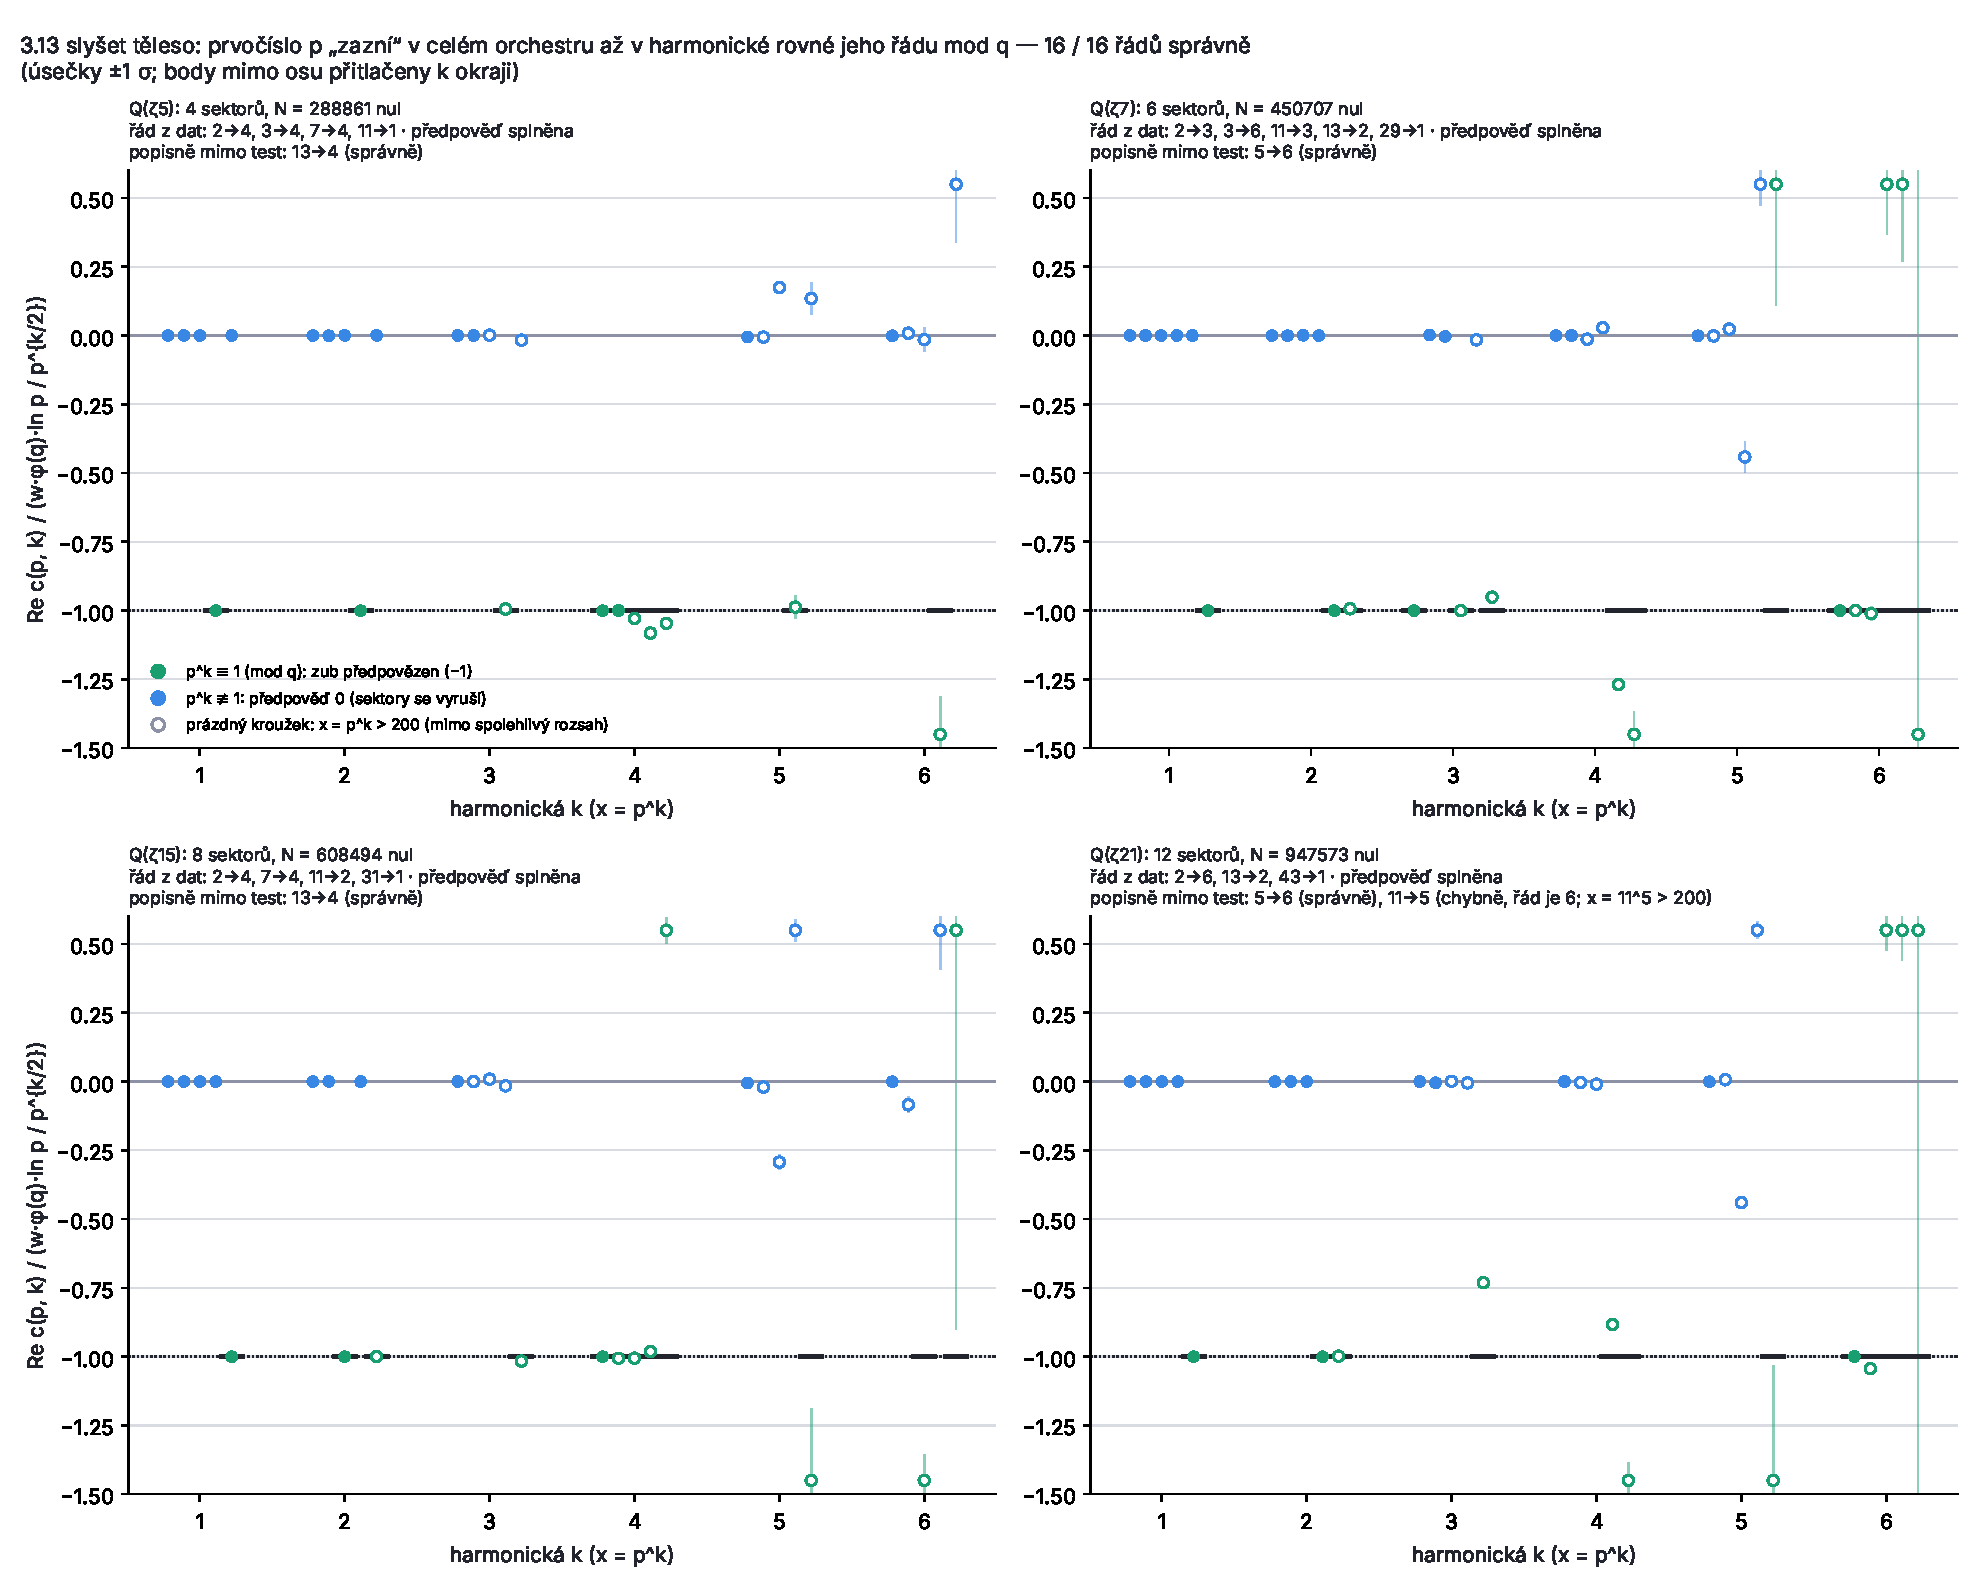
\includegraphics[width=1\textwidth,height=\textheight]{../../figures/03_body_cz.pdf}
\caption{Obrázek 3. Slyšet těleso nástroje (test 3.13): koeficienty
\(\mathrm{Re}\,c(p, k)\) sjednocení všech charakterů modulo 5, 7, 15 a
21 vztažené k plné síle zubu, proti harmonické \(k\). Plné zelené:
\(p^k \equiv 1 \pmod q\), předpověď \(-1\); plné modré: předpověď 0;
prázdné kroužky: \(x = p^k > 200\), mimo test (\(\pm 1\) chyba; body za
okrajem osy jsou nakresleny na okraji).}
\end{figure}

\hypertarget{sduxedlenuxe9-druxe1hy}{%
\subsection{4.5 Sdílené dráhy}\label{sduxedlenuxe9-druxe1hy}}

U všech 18 dvojic téhož modulu je křížová kovariance v \(\ln x = 3\)
devatenáctkrát větší než její chyba a souhlasí s prvočíselnou stopou s
relativní fází \(\chi_a(p)\overline{\chi_b(p)}\) na \(4\cdot10^{-5}\)
relativně; v \(\ln x = 4, 5, 6\) je relativní rozdíl nejvýš
\(3\cdot10^{-4}\), \(7\cdot10^{-3}\) a \(3\cdot10^{-2}\), kdežto čekaný
signál klesá na 15, 3,5 a 0,7 násobku chyby. Všechna \(|z| \le 0{,}06\):
odhad chyby (větší ze vzorce pro nezávislá okna a rozptylu přes
podpásma) je opět opatrný, takže shodu lépe popisuje relativní rozdíl. U
\(\tau = 1\) je největší normovaná křížová kovariance na mřížce hřebene
0,76--0,92 (popisně).

\hypertarget{nasycenuxed}{%
\subsection{4.6 Nasycení}\label{nasycenuxed}}

Rozptyl počtu všech patnácti L-funkcí souhlasí s dvoubodovou funkcí bez
činitelů \(p \mid q\): \(Q = 0{,}32\)--\(1{,}72\); například 21.17:
\(\Sigma^2 = 0{,}317; 0{,}401; 0{,}324\) pro
\(\ell \approx 1{,}06; 11{,}2; 91{,}1\) proti
\(0{,}317; 0{,}400; 0{,}324\). GUE dává \(Q \ge 6\,500\), naivní
předpověď \(Q \ge 81\) a Berryho diagonální vzorec, který je přesný jen
asymptoticky, v této výšce \(Q = 11{,}6\)--\(29{,}8\).

\hypertarget{robustnost-hlavnuxed-rezonance}{%
\subsection{4.7 Robustnost hlavní
rezonance}\label{robustnost-hlavnuxed-rezonance}}

Nuly použité v této části (pásma P8 a P3e10 Plattových tabulek, každé s
52 498 nezávislými okny) už byly viděny ve studii VI; nová jsou jen
čísla níže, takže tato část je slabší než slepý test.

\emph{Jiné okno.} S Hannovým oknem je rozptyl v \(\tau = 1\) roven
\(1{,}4330 \pm 0{,}0063\) v P8 (předpověď 1,4305, \(z = +0{,}40\); GUE
bez aritmetiky 0,9992, \(z = +69{,}4\)) a \(1{,}3943 \pm 0{,}0061\) v
P3e10 (předpověď 1,3897, \(z = +0{,}76\); GUE \(z = +64{,}9\)). Přes 201
bodů průběhu je \(Q = 0{,}66\) a \(0{,}93\) proti dvoubodové funkci a
\(737\) a \(531\) proti GUE (obr. 4).

\emph{Jiné odhady chyby.} S Gaussovým oknem studie VI a šesti odhady
chyby v \(\tau = 1\) (5, 10, 20 a 40 podpásem, \(V/\sqrt M\) a blokový
jackknife s 1 000 bloky) je vzdálenost od GUE mezi 13,4 a 69,3 chyby v
P8 a mezi 12,0 a 62,2 v P3e10; vzdálenost od dvoubodové funkce je nejvýš
0,71 a 0,92. Údaj 46,1 chyby uvedený ve studii VI je tedy jedna hodnota
z rozpětí, které určuje volba odhadu chyby. Nejmenší hodnota rozpětí je
12.

\emph{Plná kovariance.} S kovarianční maticí 201 bodů (blokový
jackknife, Hotellingova oprava) je dvoubodová funkce s daty slučitelná
(\(p = 0{,}976\) a \(0{,}978\)) a GUE není (\(p < 10^{-10}\)). Těch 201
bodů odpovídá 42 a 54 nezávislým bodům. Největší odchylka od předpovědi
přes průběh je 2,68 a 2,77 chyby; se zahrnutím hledání přes mřížku je
její globální \(p\)-hodnota 0,55 a 0,47. V kontrolních bodech mimo
rezonance (\(\tau = 0{,}5\) až \(2{,}0\)) je odchylka od předpovědi
nejvýš 1,71 a 1,05 chyby.

\emph{L-funkce.} S Hannovým oknem dávají hřebeny dvanácti L-funkcí sady
hr7 a tří reálných charakterů studie VI v témž pásmu
\(Q = 0{,}46\)--\(0{,}86\) proti předpovědi a \(14\)--\(55\) proti GUE.
S plnou kovariancí (364 oken) je \(p\) mezi 0,71 a 1,00 u čtrnácti z
patnácti a 0,042 u charakteru modulo 5 s \(\chi(2) = i\) (5.2); mez,
\(p \ge 10^{-3}\) u všech dvanácti, je splněna a jedna hodnota této
velikosti mezi patnácti není neobvyklá.

\begin{figure}
\centering
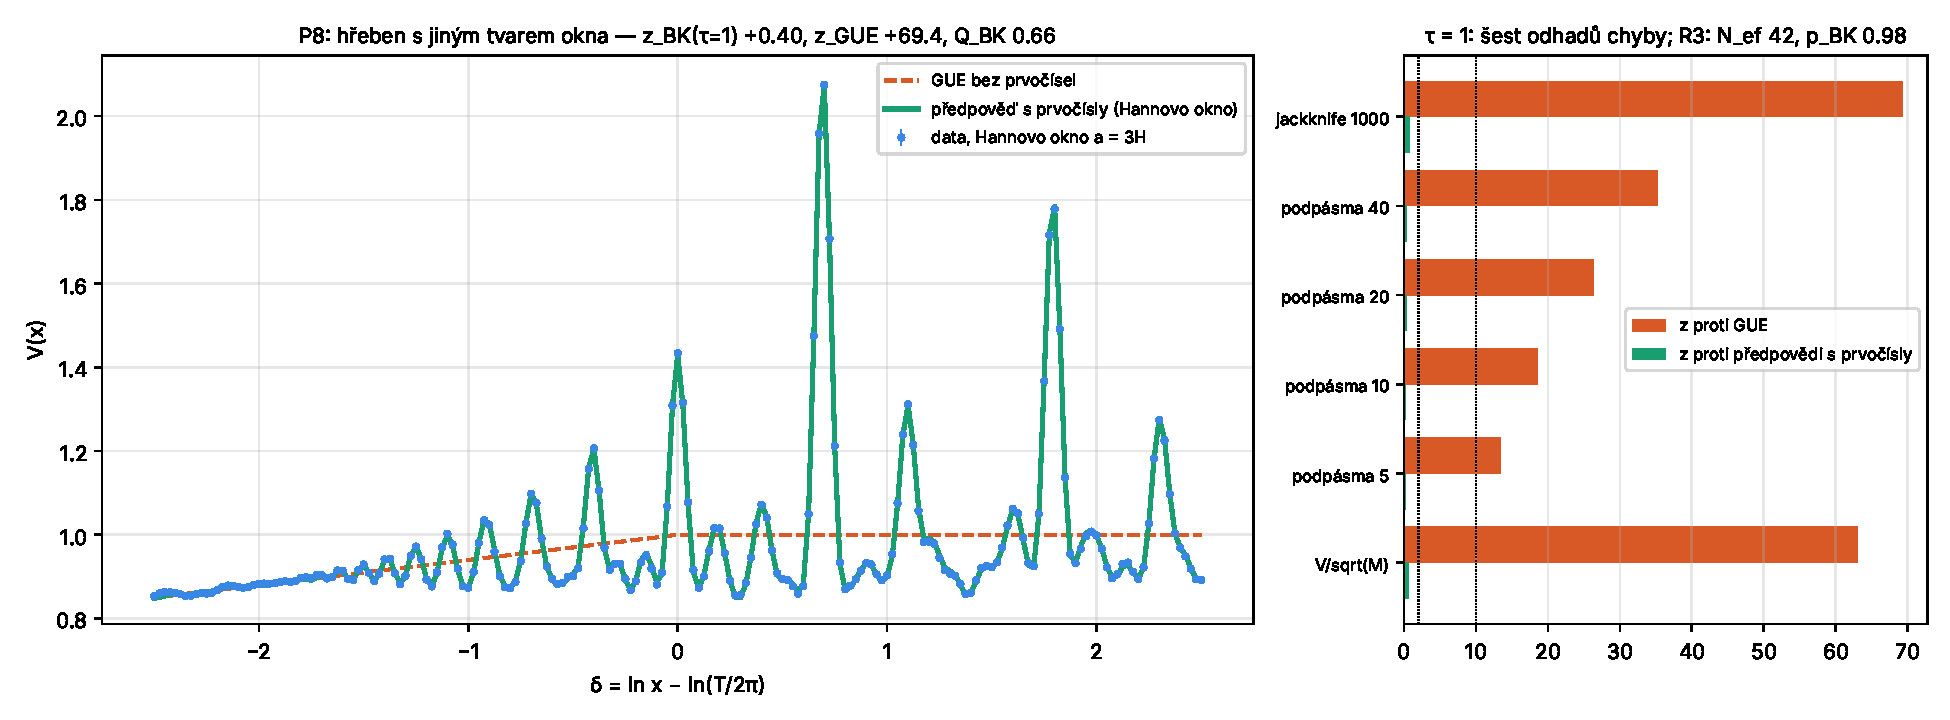
\includegraphics[width=1\textwidth,height=\textheight]{../../figures/04a_robustness_P8_cz.pdf}
\caption{Obrázek 4a. Robustnost hlavní rezonance studie VI, pásmo P8
(\(t \approx 10^8\)). Vlevo: hřeben s Hannovým oknem proti dvoubodové
funkci a GUE bez aritmetiky. Vpravo: vzdálenost od GUE a od předpovědi v
\(\tau = 1\) pro šest odhadů chyby.}
\end{figure}

\begin{figure}
\centering
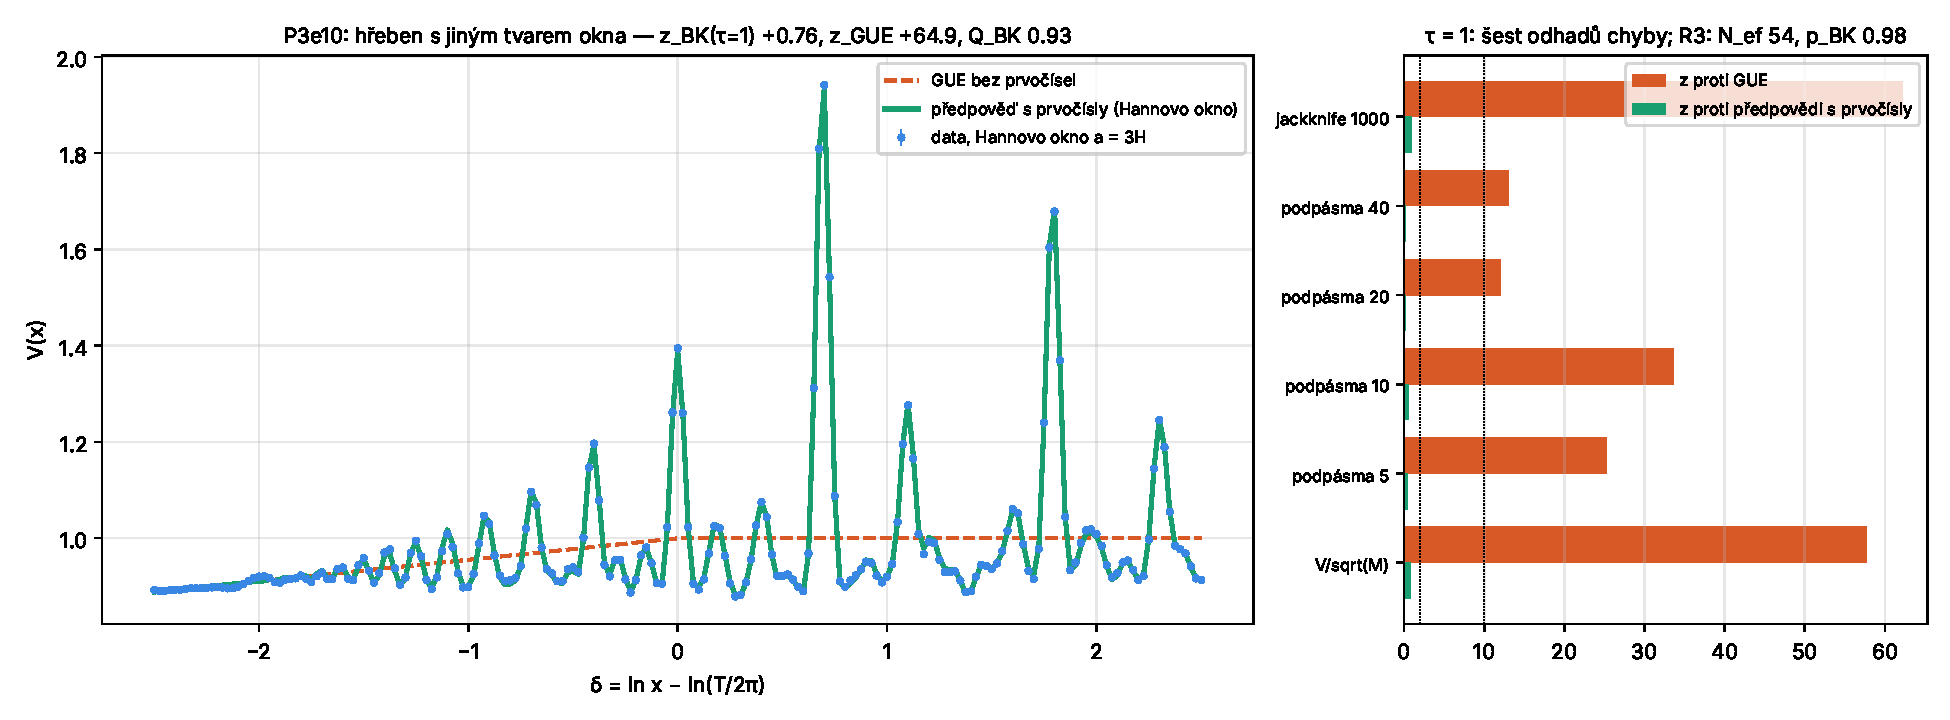
\includegraphics[width=1\textwidth,height=\textheight]{../../figures/04b_robustness_P3e10_cz.pdf}
\caption{Obrázek 4b. Totéž pro pásmo P3e10
(\(t \approx 3\cdot10^{10}\)).}
\end{figure}

\hypertarget{slyux161et-nuxe1stroj-ladux11bnuxed-a-tux11bleso}{%
\subsection{4.8 Slyšet nástroj, ladění a
těleso}\label{slyux161et-nuxe1stroj-ladux11bnuxed-a-tux11bleso}}

Tři slepé testy, určené i s mezemi v dodatcích 5 a 6 dřív, než byla data
vyhodnocena, dělají z výsledků výše použití. Popsány jsou s hudebním
čtením v oddílu 5; čísla jsou tato. Jen z koeficientů prvního řádu byl
určen modul i charakter u 16 ze 16 L-funkcí, se skóre nejvýš
\(1{,}1\cdot10^{-6}\) proti 6,0 nebo více u dalšího kandidáta (nejmenší
hodnota 5,999) (oddíl 5.4). Jen z hřebene byla určena prvočísla z 2, 3,
5, 7, která dělí modul, u 16 ze 16 (\(Q = 0{,}13\)--\(0{,}78\), další
podmnožina \(2{,}25\)--\(10{,}97\); oddíl 5.5, obr. 5). Ze sjednocení
všech charakterů modulu byl řád prvočísla přečten správně u všech 16
prvočísel určených předem ve čtyřech kruhových tělesech (oddíl 5.6, obr.
3).

\begin{figure}
\centering
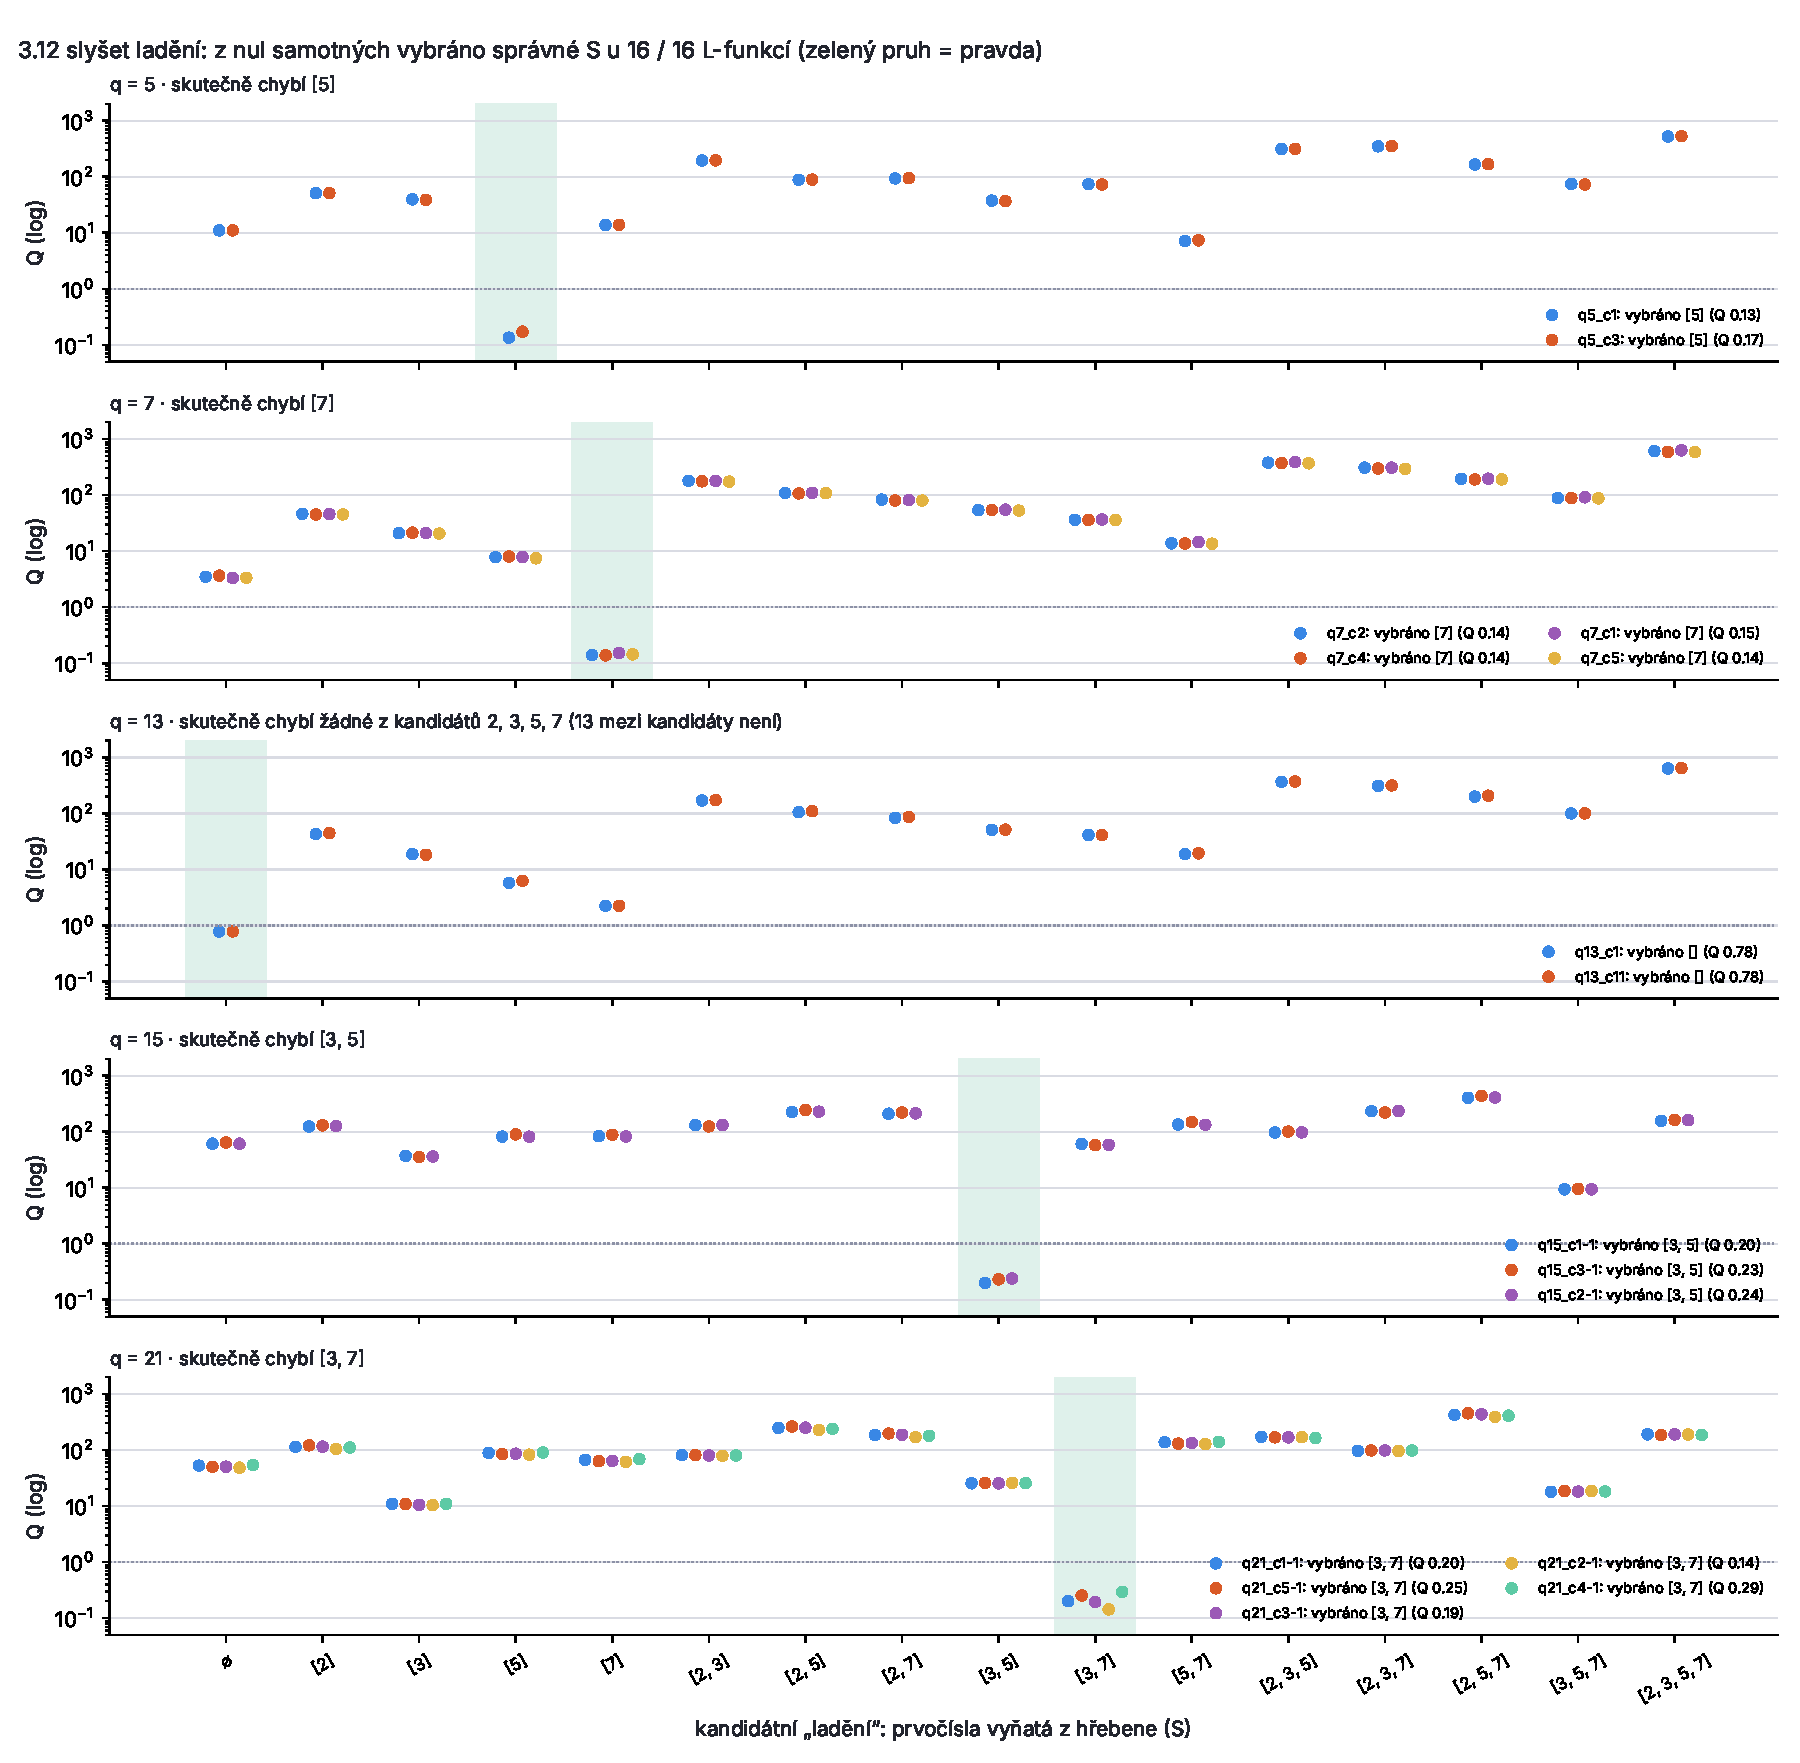
\includegraphics[width=1\textwidth,height=\textheight]{../../figures/05_tuning_cz.pdf}
\caption{Obrázek 5. Slyšet ladění (test 3.12): \(Q\) hřebene každé z 16
L-funkcí proti předpovědi bez prvočísel podmnožiny \(S\) množiny
\(\{2, 3, 5, 7\}\); zvýrazněný pruh označuje prvočísla, která dělí
modul.}
\end{figure}

\hypertarget{certifikace}{%
\subsection{4.9 Certifikace}\label{certifikace}}

Deset oken každé L-funkce rozložených přes pásmo (okna začínající v 36
000, 40 400, \ldots, 75 600; 120 oken, 21 707 nul) bylo certifikováno
intervalovou aritmetikou (Arb přes python-flint {[}21{]}): u každé nuly
bylo s rigorózními mezemi chyby ověřeno, že Hardyho funkce
\(Z(t, \chi)\) mění znaménko mezi sousedními středy, při pracovní
přesnosti nejvýš 80 bitů (kontrola K1). Deset nejtěsnějších dvojic každé
L-funkce v rozvinutém rozestupu (120 dvojic; nejmenší rozvinutý rozestup
0,0071, nejmenší rozestup \(3{,}9\cdot10^{-3}\)) bylo odděleno týmž
způsobem (K4). Přepočet dvou oken každé L-funkce (36 000--36 100 a 58
000--58 100) na stolním počítači v PARI s pracovní přesností 38 číslic
místo 19 (K2) a se čtyřikrát jemnějším vyhledávacím krokem (K3) dal
stejné počty a polohy do \(5{,}1\cdot10^{-11}\) (48 přepočtů pro sadu
hr7, 16 pro čtyři L-funkce přidané kvůli tělesům
\(\mathbb{Q}(\zeta_{15})\), \(\mathbb{Q}(\zeta_{21})\)). Tyto kontroly
nevidí dvojici velmi těsných nul přeskočenou v jiném okně; kvůli tomu
byl přidán test počtu Turingova typu (oddíl 4.10).

\hypertarget{uxfaplnost-dvux11b-pux159eskoux10denuxe9-dvojice-tux11bsnuxfdch-nul}{%
\subsection{4.10 Úplnost: dvě přeskočené dvojice těsných
nul}\label{uxfaplnost-dvux11b-pux159eskoux10denuxe9-dvojice-tux11bsnuxfdch-nul}}

Nuly se hledaly ze změn znaménka Hardyho funkce na mřížce jedné
dvaatřicetiny středního rozestupu, se zjemněním jen tehdy, když oknu
šířky 100 chybělo do hladkého počtu víc než 1,5 nuly. Před vyhodnocením
sady hr7b byl přidán další test (dodatek 7 k pravidlům): s
\(r_n = \theta_\chi(\gamma_n)/\pi - n\) se chybějící nula projeví
trvalým skokem \(r_n\) o \(+1\). Průměr \(r_n\) přes 400 následujících
nul minus průměr přes 400 předchozích zůstává do 0,01 u všech dvanácti
L-funkcí sady hr7, které jsou tedy úplné. V sadě hr7b ukázal skok
\(+2{,}00\) ve dvou oknech: dvojice nul vzdálených \(9\cdot10^{-3}\) u
\(\gamma \approx 62\,027{,}74\) pro charakter 15.14 a dvojice vzdálená
\(1{,}0\cdot10^{-2}\) u \(\gamma \approx 51\,751{,}58\) pro 21.11 byly
přeskočeny. Počty obou oken byly pod hladkým počtem o 1,49 a o 0,95
nuly, takže se zjemnění nespustilo; schodek této velikosti je v mezích
běžného kolísání \(S(t)\) a počet v jediném okně chybějící dvojici
odhalit nemůže. Obě okna byla na stolním počítači spočtena znovu se
čtyřikrát jemnější mřížkou: v každém přibyly právě ty dvě nuly, žádná
nula se nezměnila a nezávislý přepočet v cloudu je shodný bit po bitu.
Po opravě nezůstává skok u žádné ze 16 L-funkcí. Testy oddílu 5 byly
spuštěny až poté, s jednou výjimkou uvedenou v oddílu 5.4.

\hypertarget{rozliux161enuxed-co-slyux161uxed-sjednocenuxed-u-115-a-116}{%
\subsection{\texorpdfstring{4.11 Rozlišení: co slyší sjednocení u
\(11^5\) a
\(11^6\)}{4.11 Rozlišení: co slyší sjednocení u 11\^{}5 a 11\^{}6}}\label{rozliux161enuxed-co-slyux161uxed-sjednocenuxed-u-115-a-116}}

Tato analýza vznikla po vyhodnocení (dodatek 8 k pravidlům) a je
popisná. Součet přes nuly pásma šířky \(\Delta T\) oddělí dvě čísla
\(x\) a \(x + d\) jen tehdy, když
\(d \gtrsim 2\pi x/\Delta T \approx x/7000\): 0,03 u \(x = 200\), ale 23
u \(11^5\) a 253 u \(11^6\). Ve sjednocení modulo 21 zní každá mocnina
prvočísla \(n \equiv 1 \pmod{21}\) s vahou
\(\varphi(21)\Lambda(n)/\sqrt n\) a prvočíslo 161 071 \(\equiv 1\) leží
20 nad \(11^5 = 161\,051 \equiv 2\). S Gaussovou vahou přes celé pásmo
(\(T_0 = 58\,000\), \(H = 4\,000\)) byl součet
\(Z(x) = \sum_\gamma g(\gamma)x^{i\gamma}\) přes 947 573 nul sjednocení
porovnán s explicitním vzorcem sečteným přes mocniny prvočísel u \(x\),
bez volného parametru, v \(11^k\) (\(k \le 6\)) a na 1 602 bodech kolem
\(11^5\) a \(11^6\) (obr. 6): souhlasí na \(1{,}9\cdot10^{-10}\) celkové
váhy, tedy na \(1{,}2\cdot10^{-6}\) plné síly zubu prvočísla 11. U
\(11^5\) je měřená hodnota 4,42 násobku této síly a celá pochází od 161
071; po odečtení sousedních prvočísel je zbytek \(2\cdot10^{-7}\), takže
11 v páté harmonické mlčí, jak má. U \(11^6 = 1\,771\,561 \equiv 1\) je
zub prvočísla 11 překryt prvočísly \(\equiv 1 \pmod{21}\) kolem něj (55
do vzdálenosti 5 800, nejbližší 126 daleko); po jejich odečtení je
zbytek \(-1{,}000001\), zub prvočísla 11 v plné síle. Odečtení používá
seznam prvočísel, takže je to kontrola explicitního vzorce, a ne čtení z
nul samotných.

U \(11^5\) je čtení jen z nul a z modulu ještě možné, protože šířka
jádra (40) je srovnatelná s roztečí lichých kandidátů
\(n \equiv 1 \pmod{21}\) (42): proložení nejmenšími čtverci s neznámými
amplitudami u těchto kandidátů a se zkušebním členem v samotném \(11^5\)
(29 neznámých, číslo podmíněnosti \(1{,}8\cdot10^7\)) vrací amplitudu
zkušebního členu \(3\cdot10^{-6}\) plné síly a mezi 14 kandidáty do
vzdálenosti 300 od \(11^5\) vrací pět prvočísel s amplitudou
\(1 \pm 4\cdot10^{-7}\) a devět složených čísel s nejvýš
\(5\cdot10^{-7}\). U \(11^6\) je jádro desetkrát širší než rozteč a
takové čtení v tomto pásmu možné není; přečíst řád 6 z nul samotných by
vyžadovalo pásmo asi desetkrát širší.

\begin{figure}
\centering
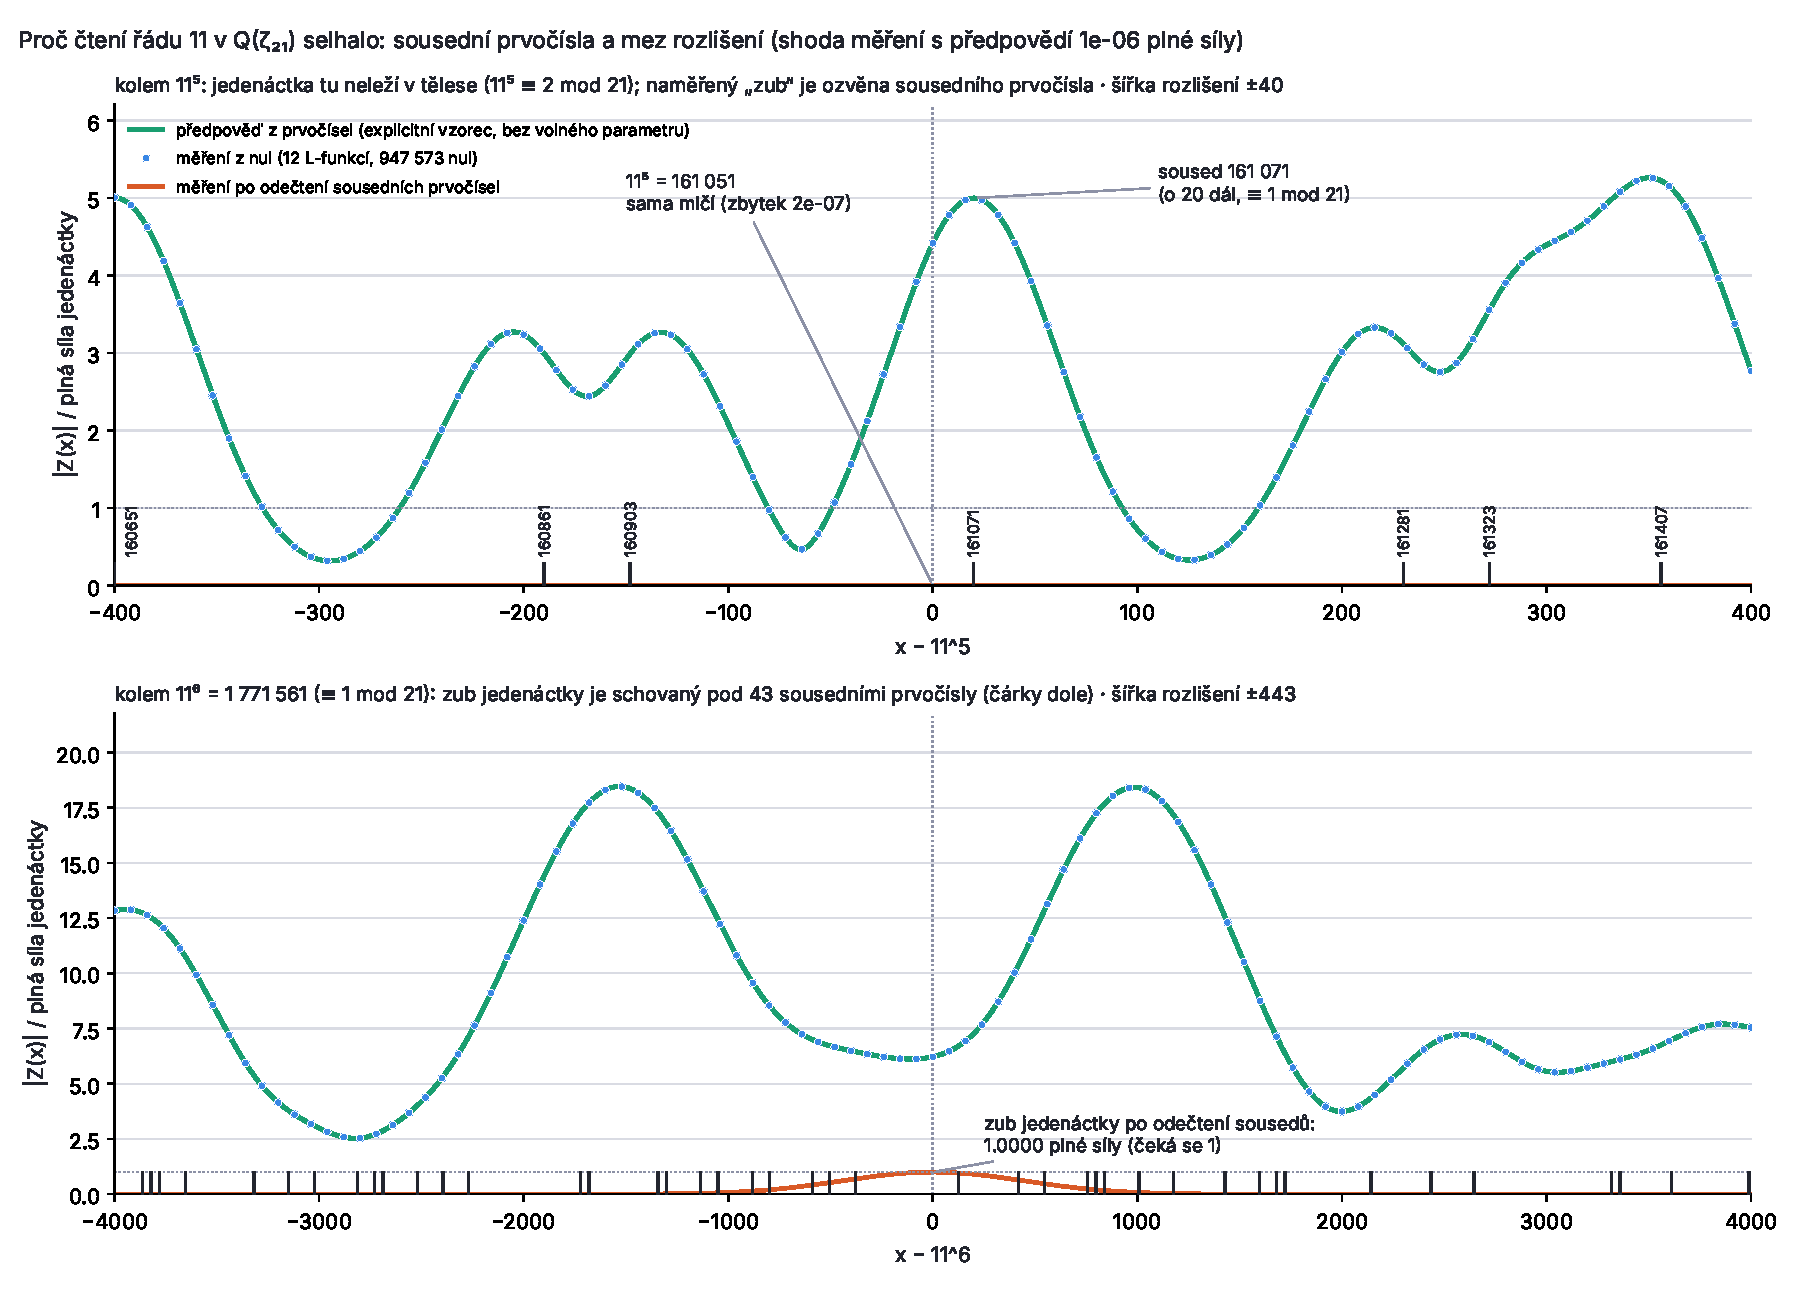
\includegraphics[width=1\textwidth,height=\textheight]{../../figures/06_resolution_cz.pdf}
\caption{Obrázek 6. Rozlišení u \(11^5\) a \(11^6\) ve sjednocení modulo
21: \(|Z(x)|\) z 947 573 nul sjednocení (body) proti explicitnímu vzorci
sečtenému přes mocniny prvočísel blízko \(x\) (čára), v jednotkách plné
síly zubu jedenáctky, a zbytek po odečtení sousedních prvočísel; čárky
označují prvočísla \(\equiv 1 \pmod{21}\).}
\end{figure}

\hypertarget{kde-konux10duxed-nuxe1hodnuxe9-matice-puxe1rovuxe1-korelace-jednuxe9-l-funkce}{%
\subsection{4.12 Kde končí náhodné matice: párová korelace jedné
L-funkce}\label{kde-konux10duxed-nuxe1hodnuxe9-matice-puxe1rovuxe1-korelace-jednuxe9-l-funkce}}

U všech 16 L-funkcí popisuje párovou korelaci do tří středních rozestupů
dvoubodová funkce z {[}8{]}: \(\chi^2\) na koš 0,78--1,86 proti mezi
2,0. Samotný tvar GUE dává 6,3--16,5. V polovině středního rozestupu
leží měřené \(R_2\) pod hodnotou GUE o 0,032--0,076; předpověď je
0,045--0,065 podle modulu. Největší odchylka jednoho koše od předpovědi
je 2,3--4,0 chyby. V této výšce je tedy samotný tvar náhodných matic
viditelně neúplný už na nejkratších vzdálenostech a aritmetická oprava
rozdíl vysvětluje (obr. 7).

Popisně: rozdělení rozestupů sousedních nul u 1 296 642 rozestupů všech
16 L-funkcí dohromady se od rozdělení GUE liší až o 0,083 (u
\(s = 1{,}15\)): malých rozestupů je méně (\(-0{,}06\) u
\(s = 0{,}45\)), rozestupů kolem středu víc (\(+0{,}08\) u
\(s = 1{,}0\)--\(1{,}2\)) a velkých méně (\(-0{,}03\) u \(s = 1{,}8\)).
Spektrum je tužší než GUE. Žádná velikost unitární matice nereprodukuje
rozdělení v mezích chyb: \(\chi^2\) na koš je 156 pro \(N = 3\), 304 pro
\(N = 4\), 1 931 pro \(N = 2\) a 1 180 pro GUE, kdežto efektivní
velikost čtená z předpovězeného \(R_2\) u nuly je 2,0--2,3. Při
\(\ln(q\gamma/2\pi) \approx 11\)--\(12\) tedy jedna efektivní velikost
matice rozestupy dostatečně nepopisuje; dvoubodová teorie párovou
korelaci popisuje. (Hodnoty \(\chi^2\) rozdělení rozestupů pro
jednotlivé L-funkce neuvádíme: některé koše mají nulový rozptyl bloků.)

\begin{figure}
\centering
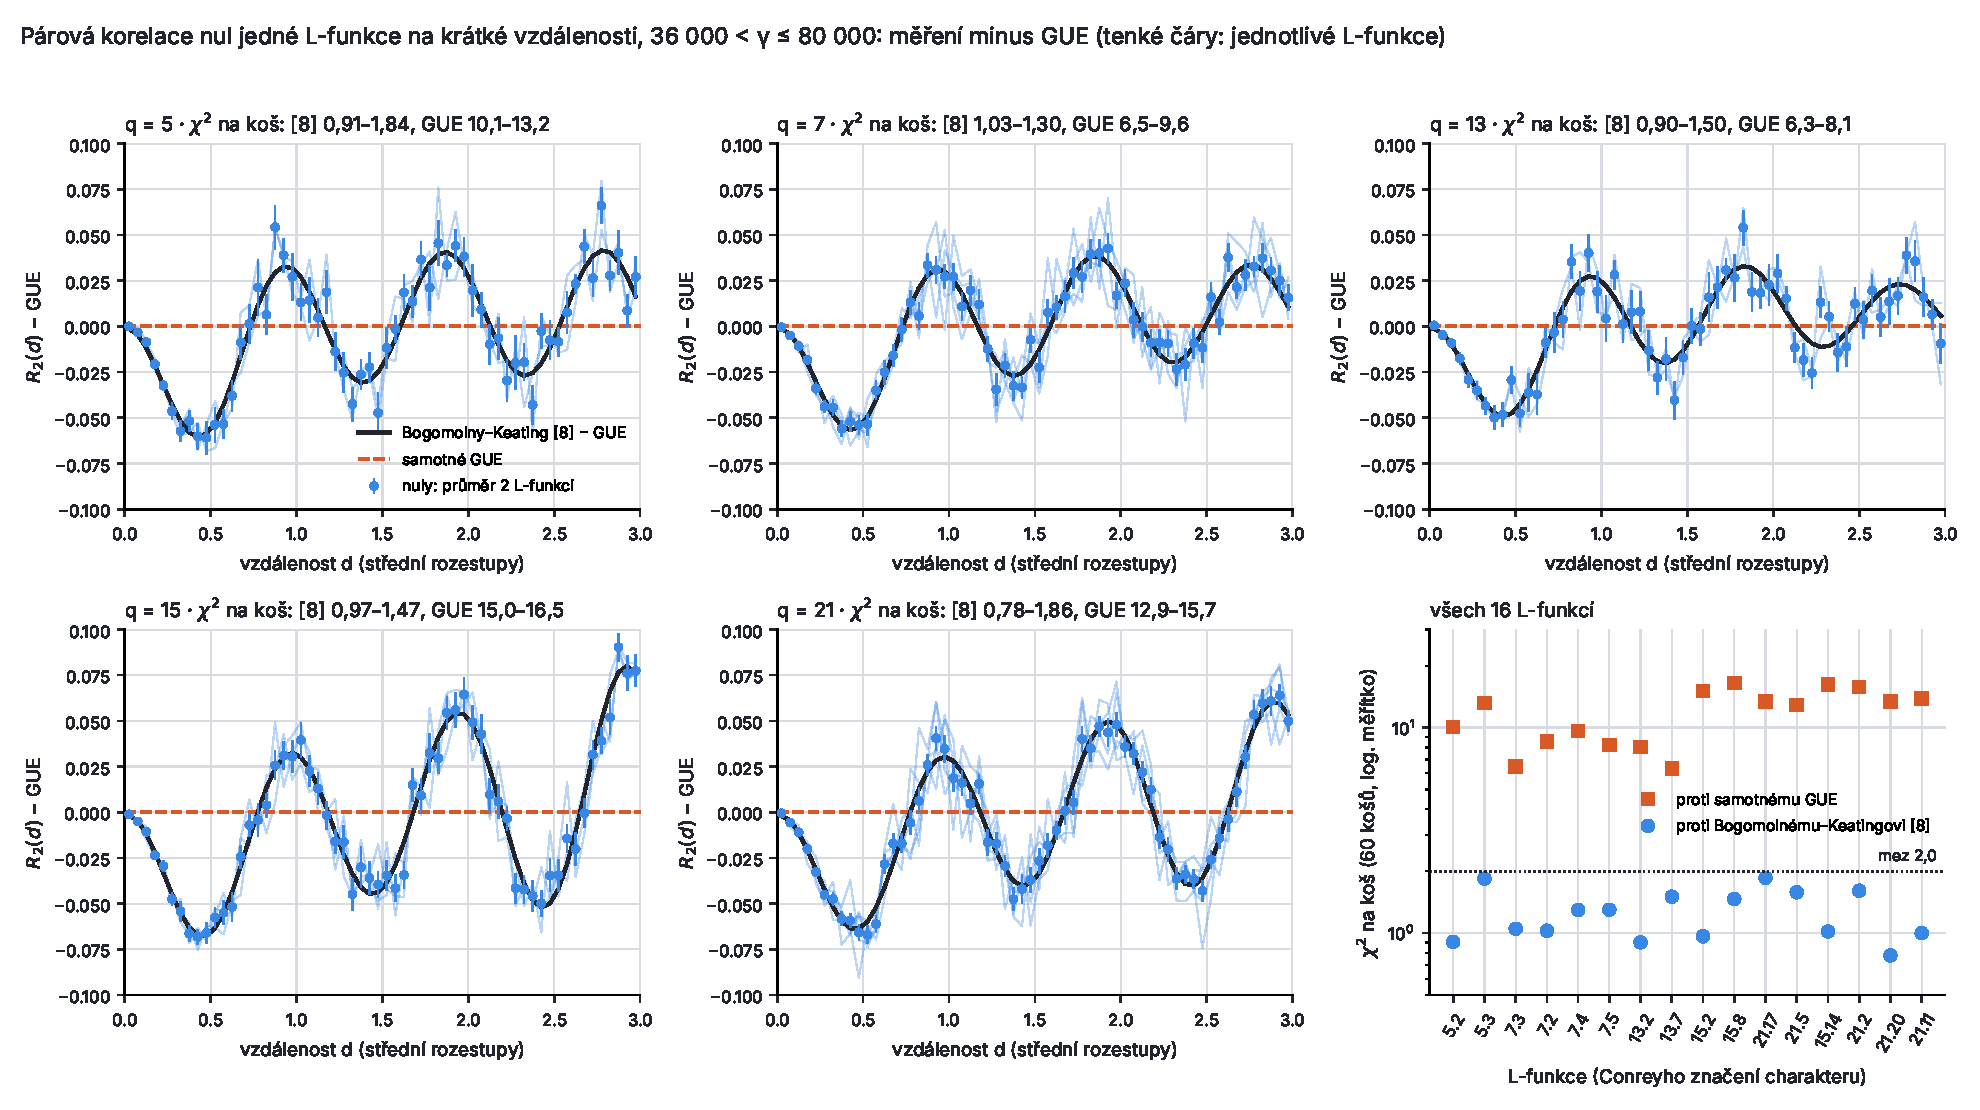
\includegraphics[width=1\textwidth,height=\textheight]{../../figures/07_pair_correlation_cz.pdf}
\caption{Obrázek 7. Párová korelace jednotlivých L-funkcí minus tvar
GUE, \(36\,000 < \gamma \le 80\,000\): data (\(\pm 1\) chyba) proti
dvoubodové funkci {[}8{]} podle modulu (tenké čáry: jednotlivé
L-funkce). Vpravo dole: \(\chi^2\) na koš všech 16 L-funkcí proti
{[}8{]} a proti samotnému GUE s mezí.}
\end{figure}

\hypertarget{orchestr-jako-sloux17eenuxed-nezuxe1visluxfdch-spekter}{%
\subsection{4.13 Orchestr jako složení nezávislých
spekter}\label{orchestr-jako-sloux17eenuxed-nezuxe1visluxfdch-spekter}}

{\small\begin{longtable}[]{@{}
  >{\raggedright\arraybackslash}p{(\columnwidth - 14\tabcolsep) * \real{0.1486}}
  >{\raggedright\arraybackslash}p{(\columnwidth - 14\tabcolsep) * \real{0.0676}}
  >{\raggedright\arraybackslash}p{(\columnwidth - 14\tabcolsep) * \real{0.1081}}
  >{\raggedright\arraybackslash}p{(\columnwidth - 14\tabcolsep) * \real{0.0946}}
  >{\raggedright\arraybackslash}p{(\columnwidth - 14\tabcolsep) * \real{0.2973}}
  >{\raggedright\arraybackslash}p{(\columnwidth - 14\tabcolsep) * \real{0.0946}}
  >{\raggedright\arraybackslash}p{(\columnwidth - 14\tabcolsep) * \real{0.0946}}
  >{\raggedright\arraybackslash}p{(\columnwidth - 14\tabcolsep) * \real{0.0946}}@{}}
\toprule\noalign{}
\begin{minipage}[b]{\linewidth}\raggedright
sjednocení
\end{minipage} & \begin{minipage}[b]{\linewidth}\raggedright
sektorů
\end{minipage} & \begin{minipage}[b]{\linewidth}\raggedright
nul
\end{minipage} & \begin{minipage}[b]{\linewidth}\raggedright
největší \(|p - p_S|\)
\end{minipage} & \begin{minipage}[b]{\linewidth}\raggedright
první koš: měřeno / \(p_S\) / Poisson
\end{minipage} & \begin{minipage}[b]{\linewidth}\raggedright
největší vzdálenost od jednoho GUE
\end{minipage} & \begin{minipage}[b]{\linewidth}\raggedright
\(\chi^2\) na koš proti \(p_S\)
\end{minipage} & \begin{minipage}[b]{\linewidth}\raggedright
košů nad 3 chyby (ze 40)
\end{minipage} \\
\midrule\noalign{}
\endhead
\bottomrule\noalign{}
\endlastfoot
\(\mathbb{Q}(\zeta_5)\) & 4 & 288 861 & 0,0096 & 0,721 / 0,731 / 0,952 &
0,71 & 3,4 & 3 \\ \addlinespace[2pt]
\(\mathbb{Q}(\zeta_7)\) & 6 & 450 707 & 0,0075 & 0,798 / 0,805 / 0,952 &
0,79 & 4,9 & 3 \\ \addlinespace[2pt]
\(\mathbb{Q}(\zeta_{15})\) & 8 & 608 494 & 0,0068 & 0,837 / 0,842 /
0,952 & 0,83 & 3,2 & 2 \\ \addlinespace[2pt]
\(\mathbb{Q}(\zeta_{21})\) & 12 & 947 573 & 0,0073 & 0,872 / 0,879 /
0,952 & 0,86 & 1,9 & 0 \\ \addlinespace[2pt]
\end{longtable}}

Všechny tři meze jsou splněny u všech čtyř sjednocení: nuly Dedekindovy
zeta funkce kruhového tělesa mají v tomto pásmu rozestupy jako složení
nezávislých spekter GUE, jednoho pro každý charakter, a ne jako jedno
spektrum GUE ani jako Poissonův proces (obr. 8), jak se čeká podle
{[}30{]} a {[}24{]}. Shoda není dokonalá. \(\chi^2\) na koš proti
\(p_S\) je 1,9--4,9 a největší jednotlivá odchylka je 2,9--8,3 chyby; v
prvním koši je měřená hustota pod \(p_S\) u všech čtyř sjednocení, o
0,006--0,010. Nejmenších rozestupů je tedy o něco méně, než by dala
nezávislá spektra. Znaménko odpovídá křížové kovarianci z oddílu 4.5
(sektory jednoho modulu sdílejí prvočísla), ale velikost tohoto jevu
spočtena nebyla a nic se o ní netvrdí. Model \(p_S\) je na výšku uvnitř
pásma necitlivý (nejvýš 0,0002).

\begin{figure}
\centering
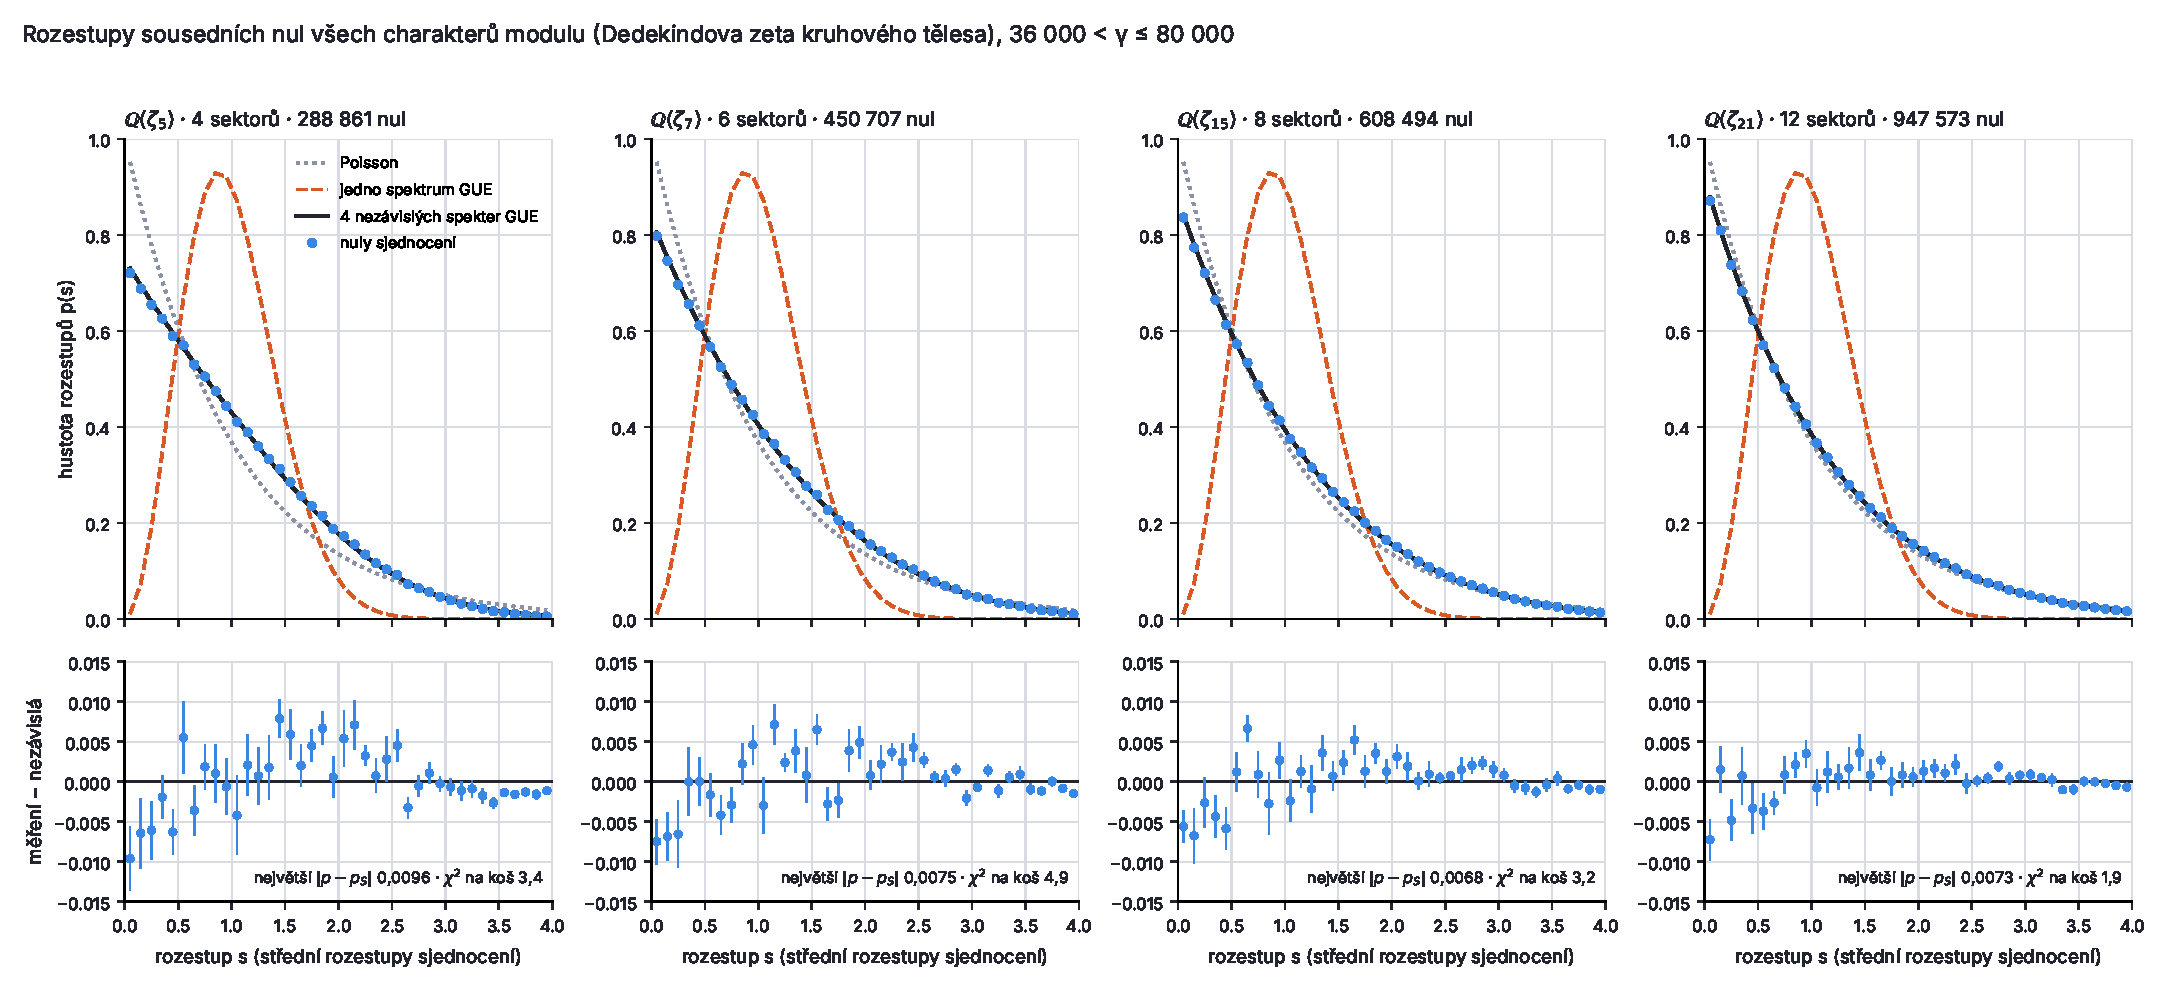
\includegraphics[width=1\textwidth,height=\textheight]{../../figures/08_unions_cz.pdf}
\caption{Obrázek 8. Hustoty rozestupů čtyř sjednocení (nuly
Dedekindových funkcí zeta těles \(\mathbb{Q}(\zeta_5)\),
\(\mathbb{Q}(\zeta_7)\), \(\mathbb{Q}(\zeta_{15})\),
\(\mathbb{Q}(\zeta_{21})\)) proti složení nezávislých spekter GUE,
jednomu spektru GUE a Poissonovu procesu; dolní panely: naměřená hustota
minus složení (\(\pm 1\) chyba).}
\end{figure}

\hypertarget{vuxfdux161ka-sluxe1bne-odchylka-od-nuxe1hodnuxfdch-matic-tak-jak-ux159uxedkuxe1-pux159edpovux11bux10f}{%
\subsection{4.14 Výška: slábne odchylka od náhodných matic tak, jak říká
předpověď?}\label{vuxfdux161ka-sluxe1bne-odchylka-od-nuxe1hodnuxfdch-matic-tak-jak-ux159uxedkuxe1-pux159edpovux11bux10f}}

Ve druhém pásmu, \(400\,000 < \gamma \le 420\,000\), mají čtyři L-funkce
sady hr7b po 43 907 až 44 980 nulách, celkem 178 844. Počty se liší od
hladkého počtu o \(-0{,}65\) až \(+1{,}35\) a test počtu z oddílu 4.10
neukazuje žádný skok (největší \(|\Delta|\) 0,01). Šest náhodně
vybraných nul každé L-funkce (celkem 24) dává v mpmath
\(|L(\tfrac12 + i\gamma, \chi)| \le 5{,}4\cdot10^{-9}\), proti nejméně
0,21 ve středech k sousední nule.

Párová korelace v tomto pásmu opět sleduje dvoubodovou funkci z {[}8{]}:
\(\chi^2\) na koš 1,05--1,82, proti 3,5--8,0 u samotného GUE (obr. 9).
Amplituda měřené odchylky od GUE ve tvaru předpovědi je 0,92--1,07 u
čtyř L-funkcí a \(0{,}987 \pm 0{,}027\) sdruženě (1 znamená přesně podle
předpovědi; v dolním pásmu \(0{,}995 \pm 0{,}011\)). Velikost odchylky
klesá z \(0{,}0363 \pm 0{,}0004\) v dolním pásmu na
\(0{,}0261 \pm 0{,}0007\) v horním, rozdíl je 12,6 chyby. Poměr obou
velikostí je \(0{,}719 \pm 0{,}021\); předpověď bez volného parametru je
0,727. Všechny čtyři meze jsou splněny. Mezi
\(L = \ln(qT/2\pi) \approx 12{,}2\) a \(14{,}1\) (pro \(q = 21\)) se
tedy odchylka zmenšuje zhruba jako \(1/L^2\), jak říká dvoubodová
funkce, a její tvar zůstává stejný. Popisně: největší rozdíl rozdělení
rozestupů sousedních nul od GUE je u týchž čtyř L-funkcí 0,071--0,081 v
horním pásmu a 0,082--0,106 v dolním.

\begin{figure}
\centering
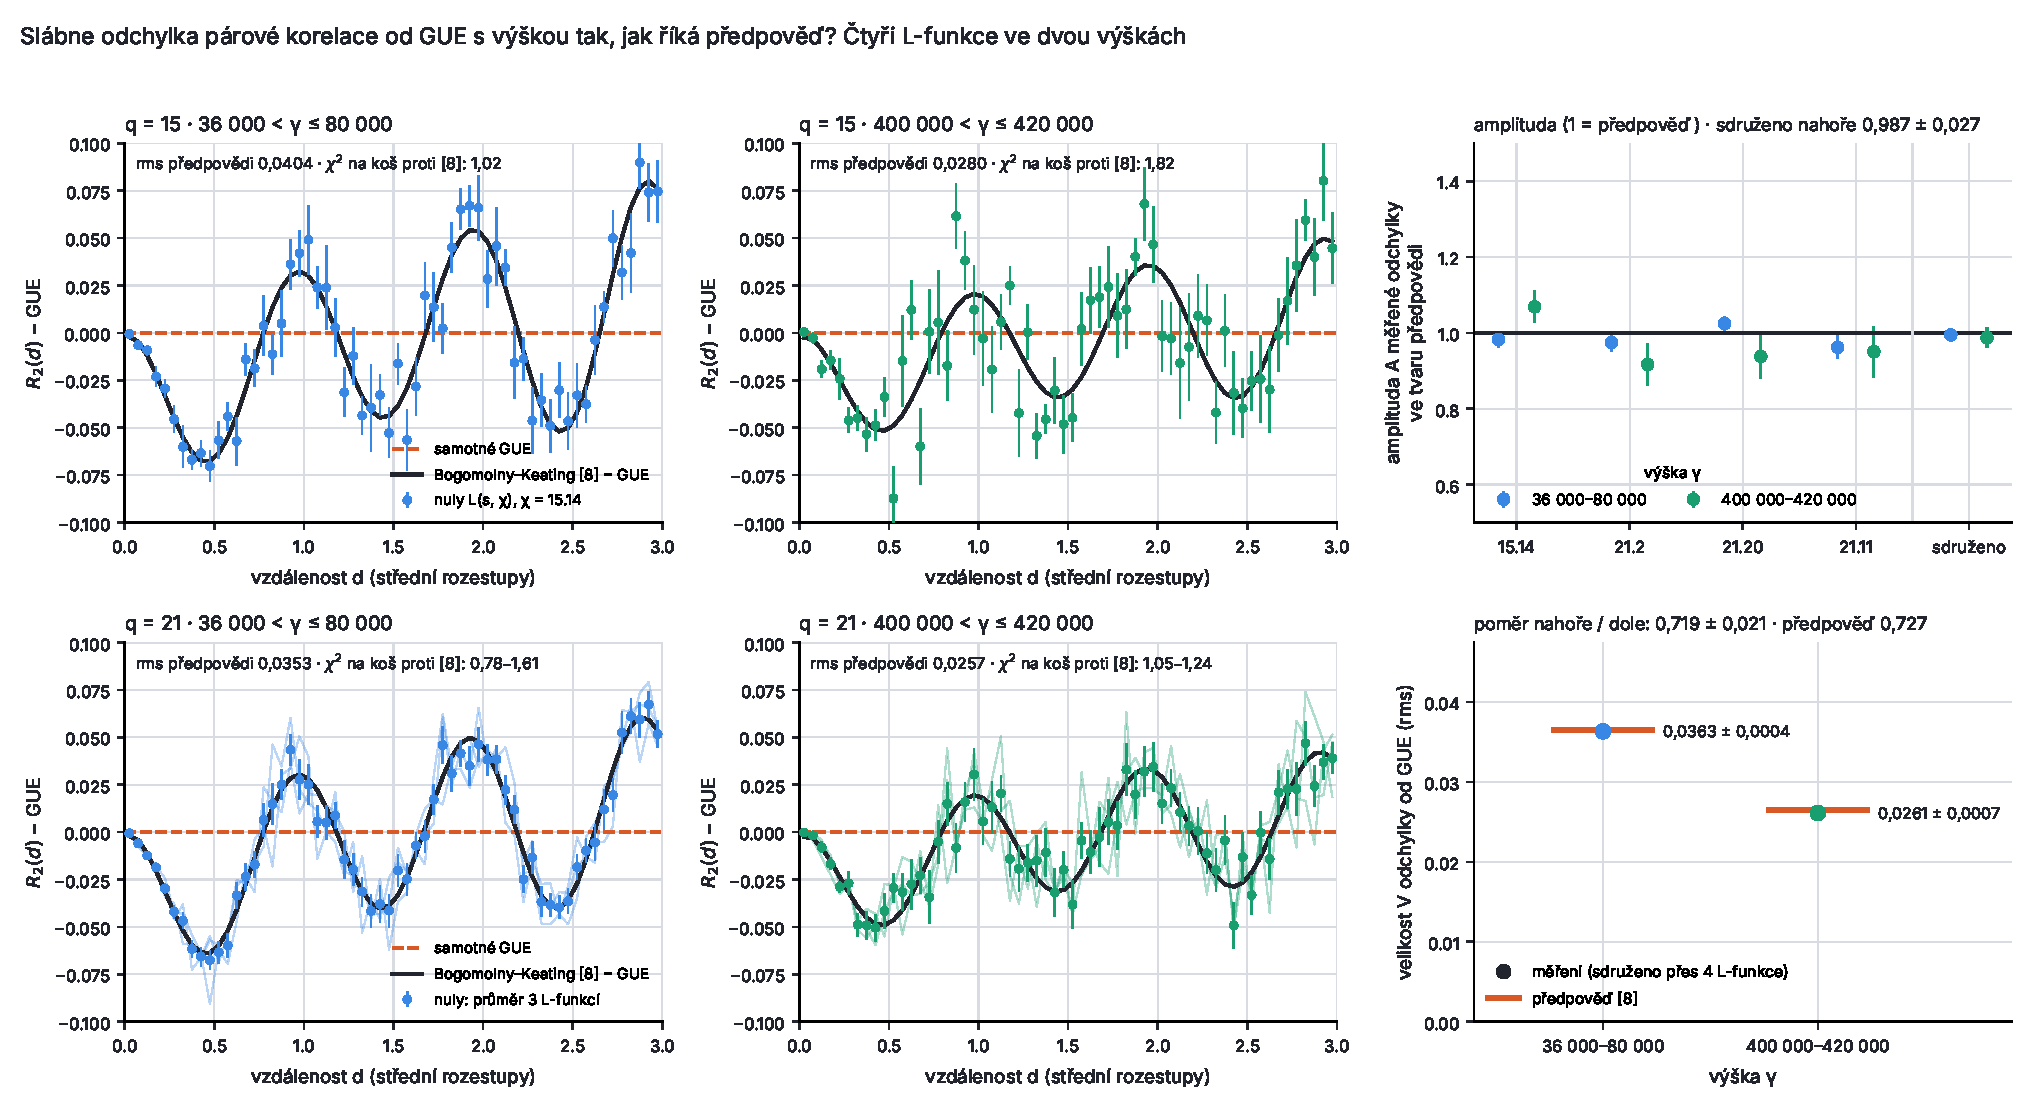
\includegraphics[width=1\textwidth,height=\textheight]{../../figures/09_height_cz.pdf}
\caption{Obrázek 9. Výška. Párová korelace minus GUE pro L-funkce sady
hr7b v pásmech 36 000--80 000 a 400 000--420 000 proti dvoubodové funkci
{[}8{]}; amplituda naměřené odchylky podél předpovězeného tvaru pro
každou L-funkci a sdruženě; velikost odchylky v obou pásmech proti
předpovědi.}
\end{figure}

\hypertarget{hudebnuxed-ux10dtenuxed-a-jak-ho-pouux17euxedt}{%
\section{5. Hudební čtení a jak ho
použít}\label{hudebnuxed-ux10dtenuxed-a-jak-ho-pouux17euxedt}}

V této řadě slouží jazyk hudby jako pomůcka ke čtení měření, ne jako
tvrzení o zvuku. Každý výrok níže má přesný protějšek ve vzorcích oddílu
3 a každý test „slyšení`` byl i se svou mezí určen dřív, než byla data
vyhodnocena.

\hypertarget{harmonickuxe1-ux159ada}{%
\subsection{5.1 Harmonická řada}\label{harmonickuxe1-ux159ada}}

Struna zní na základním kmitočtu a na jeho celočíselných násobcích,
alikvótních tónech. V explicitním vzorci hrají prvočísla úlohu
základních tónů s „délkami`` \(\ln p\) a mocniny prvočísel \(p^k\) jsou
jejich alikvóty s délkami \(k\ln p\) a vahami \(\ln p/p^{k/2}\).
Koeficienty prvního řádu \(c_k(p)\) z oddílu 4.4 jsou doslova amplitudy
těchto alikvótů v nulách.

\hypertarget{prvoux10duxedselnuxe1-mez}{%
\subsection{5.2 Prvočíselná mez}\label{prvoux10duxedselnuxe1-mez}}

V čistém ladění se ladění nazývá \(P\)-limitní, když jsou všechny jeho
intervaly poměry celých čísel složených z prvočísel \(\le P\): 3-limit
je pythagorejské ladění, 5-limit přidává čistou velkou tercii 5/4.
Hřeben \(\zeta\) obsahuje intervaly \(A/B\) všech prvočísel; hřebeni
\(L(s, \chi)\) chybějí právě prvočísla dělící \(q\). Modul 15 je tedy
ladění bez 3 a 5 a jeho zub na oktávě \(A/B = 2\) je skoro dvakrát vyšší
než u \(q = 5\) (předpověď 7,15 proti 3,81, měřeno v průměru 7,13),
protože oktáva už nedělí sílu se sousedními intervaly složenými z 3 a 5.
Popisně: shoda hřebene se zlepšuje, jak se do předpovědi připouští víc
prvočísel: pro \(q = 5\) (5.2) je \(Q = 3{,}3\) jen s prvočíslem 2, 0,26
s 2 a 3 a 0,13 se všemi prvočísly; pro \(q = 15\) (15.2) 0,49 do
\(P = 5\) (přispívá jen 2), 0,31 se 7 a 0,20 se všemi; pro \(q = 21\)
(21.17) 1,0 do \(P = 3\), 0,21 od \(P = 5\) a 0,20 se všemi.

\hypertarget{komma}{%
\subsection{5.3 Komma}\label{komma}}

Dvanáct čistých kvint přesahuje sedm oktáv o pythagorejské komma
\(3^{12}/2^{19} \approx 1{,}0136\); žádná mocnina 3 se nerovná mocnině
2, protože \(\ln 3/\ln 2\) je iracionální. V hřebeni je to důvod, proč
zuby sedí jen u racionálních poměrů \(A/B\): dvě různé mocniny prvočísel
nikdy nemají stejnou délku, takže dráhy nesplynou do společného zubu.
Studie VI použila iracionální násobky jako kontrolu: pro
\(\alpha = \sqrt2/2\pi\) a \(\sqrt3/2\pi\) neukázaly zlomkové části
\(\{\gamma\alpha\}\) žádnou strukturu nad rovnoměrnou hustotu {[}6{]}.
Nové měření se zde nedělá.

\hypertarget{slyux161et-nuxe1stroj-test-3.11}{%
\subsection{5.4 Slyšet nástroj (test
3.11)}\label{slyux161et-nuxe1stroj-test-3.11}}

\textbf{Použití:} dán je jen seznam nul a má se určit, které L-funkci
patří. Jen z koeficientů prvního řádu se prvočísla s
\(|c_p| < 0{,}5\,w\ln p/\sqrt p\) berou jako dělitelé modulu; mezi všemi
primitivními charaktery modulů \(q' \le 30\) s těmito prvočíselnými
děliteli se vybere ten nejbližší k
\(\hat\chi(p) = -c_p\sqrt p/(w\ln p)\). Všech dvanáct L-funkcí sady hr7
bylo určeno správně, modul i charakter, a stejně tak čtyři L-funkce sady
hr7b: 16 ze 16, se skóre nejvýš \(1{,}1\cdot10^{-6}\) proti 6,0 nebo
více u dalšího kandidáta (nejmenší hodnota 5,999). U čtyř L-funkcí sady
hr7b byl tento výsledek na datech vidět už před opravou dvou chybějících
dvojic nul (oddíl 4.10); po opravě je stejný.

\hypertarget{slyux161et-ladux11bnuxed-test-3.12}{%
\subsection{5.5 Slyšet ladění (test
3.12)}\label{slyux161et-ladux11bnuxed-test-3.12}}

\textbf{Použití:} jen z hřebene, bez prvního řádu, určit, která malá
prvočísla dělí modul. Ze 16 podmnožin \(\{2, 3, 5, 7\}\) byla ta, jejíž
předpověď sedí hřebeni nejlépe, správná u všech 16 L-funkcí
(\(Q = 0{,}13\)--\(0{,}78\), další podmnožina
\(Q = 2{,}25\)--\(10{,}97\); obr. 5). U \(q = 15\) říká sám hřeben
„chybějí 3 a 5``, u \(q = 21\) „3 a 7``.

\hypertarget{slyux161et-tux11bleso-nuxe1stroje-test-3.13}{%
\subsection{5.6 Slyšet těleso nástroje (test
3.13)}\label{slyux161et-tux11bleso-nuxe1stroje-test-3.13}}

\textbf{Použití:} z nul celé rodiny modulu --- z orchestru --- přečíst,
jak se prvočísla rozkládají v kruhovém tělese. Ve sjednocení prvočíslo
\(p\) mlčí ve všech harmonických kromě násobků svého řádu \(f(p)\)
modulo \(q\), kde zní s plnou vahou \(\varphi(q)\): všude jinde se
sektory navzájem vyruší. Řád přečtený z dat souhlasil s aritmetickým
řádem u všech 16 prvočísel určených předem ve čtyřech tělesech
\(\mathbb{Q}(\zeta_5)\), \(\mathbb{Q}(\zeta_7)\),
\(\mathbb{Q}(\zeta_{15})\), \(\mathbb{Q}(\zeta_{21})\) (obr. 3; jediné
chybné čtení mimo test uvádí oddíl 4.4). Vynětí jednoho sektoru vyrušení
poruší (negativní kontrola, popisně). Kam až toto slyšení dosáhne,
určuje délka poslechu: dva tóny s rozdílem kmitočtů \(\Delta f\) lze
rozlišit až po době asi \(1/\Delta f\) a dvě čísla \(x\) a \(x + d\) jen
z nul přes rozsah výšek asi \(2\pi x/d\) (oddíl 4.11). S pásmem použitým
zde je rozlišeno každé celé číslo do několika tisíc; u \(11^5\) už
sjednocení nerozezná 11 od prvočísla o dvacet kroků dál, pokud se
nepoužije rozteč kandidátů, a u \(11^6\) vůbec.

\hypertarget{meze-analogie}{%
\subsection{5.7 Meze analogie}\label{meze-analogie}}

Nuly nejsou kmitočty známé fyzikální soustavy a nic zde není slyšet bez
libovolné volby, jak čísla převést na zvuk. Každý jev popsaný v tomto
oddílu plyne z vět --- z explicitního vzorce, Landauova vzorce,
ortogonality charakterů a rozkladu prvočísel v kruhových tělesech ---
nebo z domněnky o dvoubodové funkci a hudební slova žádný nový obsah
nepřidávají. Slepé testy přidávají praktickou věc: hřeben a první řád
stačí k tomu, aby se z nul poznala L-funkce, její modul a rozklad
prvočísel, což může sloužit jako kontrola spočtených tabulek nul a jako
soubor podmínek, které by každý navržený operátor pro tyto nuly musel
splnit.

\hypertarget{tvrzenuxed-a-jejich-stav}{%
\section{6. Tvrzení a jejich stav}\label{tvrzenuxed-a-jejich-stav}}

Verdikty podle pravidel: O = podpořeno (splněny všechny meze), N =
nerozhodnuto, Z = zamítnuto.

{\small\begin{longtable}[]{@{}
  >{\raggedright\arraybackslash}p{(\columnwidth - 4\tabcolsep) * \real{0.7692}}
  >{\raggedright\arraybackslash}p{(\columnwidth - 4\tabcolsep) * \real{0.1154}}
  >{\raggedright\arraybackslash}p{(\columnwidth - 4\tabcolsep) * \real{0.1154}}@{}}
\toprule\noalign{}
\begin{minipage}[b]{\linewidth}\raggedright
Tvrzení
\end{minipage} & \begin{minipage}[b]{\linewidth}\raggedright
Oddíl
\end{minipage} & \begin{minipage}[b]{\linewidth}\raggedright
Verdikt
\end{minipage} \\
\midrule\noalign{}
\endhead
\bottomrule\noalign{}
\endlastfoot
odv-hr7-hreben: hřeben jedné \(L(s, \chi)\) sleduje modul & 4.2 & O \\ \addlinespace[2pt]
odv-hr7-nastroje: stejný modul, stejný hřeben (bez teorie) & 4.2 & O \\ \addlinespace[2pt]
odv-hr7-faze: první řád nese fázi \(\chi(p)\) & 4.3 & O \\ \addlinespace[2pt]
odv-hr7-presne: explicitní vzorec s Gaussovým oknem (kvalita dat) & 4.3
& O \\ \addlinespace[2pt]
odv-hr7-diag: rozptyl harmonických v diagonálním režimu & 4.3 & O \\ \addlinespace[2pt]
odv-hr7-teleso: sjednocení kruhového tělesa \(\mathbb{Q}(\zeta_5)\),
\(\mathbb{Q}(\zeta_7)\) & 4.4 & O \\ \addlinespace[2pt]
odv-hr7-krizova: křížová kovariance sektorů = prvočíselná stopa & 4.5 &
O \\ \addlinespace[2pt]
odv-hr7-nasyceni: nasycení \(\Sigma^2\) podle modulu & 4.6 & O \\ \addlinespace[2pt]
odv-hr7-okno: jiný tvar okna (\(\zeta\), P8 a P3e10) & 4.7 & O \\ \addlinespace[2pt]
odv-hr7-podpasma: jiné odhady chyby & 4.7 & O \\ \addlinespace[2pt]
odv-hr7-kovar: plná kovariance, efektivní počet bodů & 4.7 & O \\ \addlinespace[2pt]
odv-hr7-okno-L: Hannovo okno pro dvanáct L-funkcí & 4.7 & O \\ \addlinespace[2pt]
odv-hr7-nastroj: slyšet nástroj (16 L-funkcí) & 5.4 & O \\ \addlinespace[2pt]
odv-hr7-ladeni: slyšet ladění (16 L-funkcí) & 5.5 & O \\ \addlinespace[2pt]
odv-hr7-teleso2: slyšet těleso, 16 řádů ve čtyřech tělesech & 5.6 & O \\ \addlinespace[2pt]
odv-hr7-rmt-par: párová korelace na krátké vzdálenosti sleduje {[}8{]},
ne samotné GUE (16 L-funkcí) & 4.12 & O \\ \addlinespace[2pt]
odv-hr7-rmt-orchestr: rozestupy sjednocení = složení nezávislých spekter
GUE (čtyři tělesa) & 4.13 & O \\ \addlinespace[2pt]
odv-hr7-rmt-vyska: odchylka od GUE slábne s výškou podle předpovědi &
4.14 & O \\ \addlinespace[2pt]
\end{longtable}}

\hypertarget{co-je-novuxe9-a-co-potvrzenuxe9}{%
\section{7. Co je nové a co
potvrzené}\label{co-je-novuxe9-a-co-potvrzenuxe9}}

\textbf{Měřené věty.} Fáze prvního řádu je Landauův vzorec pro
\(L(s, \chi)\) ve tvaru Goneka a Bankse {[}10{]}; vyrušení ve sjednocení
kruhového tělesa je ortogonalita charakterů spolu s rozkladem prvočísel;
křížová kovariance u malých \(x\) a explicitní vzorec s Gaussovým oknem
plynou z explicitního vzorce. Oddíly 4.3--4.5 a 4.11 jsou měření známých
tvrzení na nových datech, ne nové výsledky.

\textbf{Měřené domněnky s výslovnou předpovědí.} Dvoubodová funkce pro
Dirichletovy L-funkce {[}8{]} říká, že hřeben, nasycení rozptylu počtu i
párová korelace na krátké vzdálenosti závisejí na modulu, a ne na
charakteru. Práce {[}8{]} numerické srovnání neobsahuje a pro komplexní
charaktery jsme žádné nenašli. Že se nuly různých L-funkcí chovají jako
nezávislá spektra, zdůvodnila práce {[}30{]} a je to v souladu s
{[}24{]}; oddíl 4.13 to měří na čtyřech kruhových tělesech se 4 až 12
sektory a nachází shodu na 0,010 v hustotě rozestupů, s malým soustavným
úbytkem nejmenších rozestupů. Odchylky statistiky rozestupů \(\zeta\) od
GUE v konečné výšce a jejich popis efektivní velikostí matice jsou známy
{[}25{]}; oddíl 4.12 měří odpovídající jev u 16 Dirichletových L-funkcí
a oddíl 4.14 předpovězený pokles odchylky mezi dvěma výškami u čtyř z
nich.

\textbf{Co je podle nás přidáno.} (i) Nuly 16 Dirichletových L-funkcí
mezi výškami 36 000 a 80 000 a čtyř z nich mezi 400 000 a 420 000, s
otiskem každého okna. (ii) Hřeben pro komplexní charaktery s nulovými
modely a chybami. (iii) Tři slepé testy: modul a charakter, prvočísla
dělící modul a rozklad prvočísel v kruhovém tělese byly určeny z nul
samotných podle pravidel stanovených předem. (iv) Mez rozlišení řečená
výslovně: u \(11^5\) slyší sjednocení modulo 21 sousední prvočíslo 161
071 a explicitní vzorec toto čtení vysvětluje na \(10^{-6}\) síly zubu.
(v) Test počtu Turingova typu, který našel dvě dvojice těsných nul
přeskočené vyhledávací mřížkou, se zdokumentovanou opravou. Tento výčet
odráží naše hledání v literatuře a nemusí být úplný.

\hypertarget{omezenuxed}{%
\section{8. Omezení}\label{omezenuxed}}

Dvanáct L-funkcí má malé moduly a sahá do výšky 80 000; hřeben je u
\(\tau = 1\) rozlišen jen pro \(H = 20\). Část o robustnosti používá
nuly, které už byly viděny ve studii VI. Křížová kovariance a sjednocení
kruhového tělesa se testují jen tam, kde věty dávají přesnou předpověď;
křížová kovariance u \(\tau = 1\), kam mohou vstoupit mimodiagonální
členy s Gaussovými a Jacobiho součty, je ukázána bez předpovědi.

\hypertarget{vuxfdhled}{%
\section{9. Výhled}\label{vuxfdhled}}

Přečíst řád 6 prvočísla 11 v \(\mathbb{Q}(\zeta_{21})\) z nul samotných
vyžaduje pásmo asi desetkrát širší, než jaké je použito zde (oddíl
4.11); to je plánováno jako první bod příští studie. Úbytek nejmenších
rozestupů ve sjednoceních (oddíl 4.13) by měl plynout z křížové korelace
sektorů přes společná prvočísla a dal by se spočítat z explicitního
vzorce, včetně oblasti u \(\tau = 1\), kde zde byla křížová kovariance
ukázána bez předpovědi. U rozdělení rozestupů jedné L-funkce by se místo
jedné velikosti matice dala s daty porovnat oprava z {[}25{]} bez
Eulerových činitelů \(p \mid q\). Rodiny s více sektory a moduly s více
prvočiniteli by vyzkoušely, kam až obraz nezávislých sektorů platí.

\hypertarget{reprodukovatelnost}{%
\section{10. Reprodukovatelnost}\label{reprodukovatelnost}}

Repozitář (GitHub, archivovaný na Zenodu) obsahuje všechna čísla tohoto
článku v souborech výsledků, pravidla zapsaná předem s deseti dodatky
(česky, s daty), manifesty nul s SHA-256 každého okna (5 280 oken sady
hr7, 1 760 sady hr7b se dvěma opravenými okny a 800 sady hr7c) a kód:
skript, který počítá nuly v PARI/GP, vyhodnocovací skripty s otisky
zapsanými dřív, než byla data otevřena, skripty kontrol (intervalová
aritmetika, vyšší přesnost, jemnější vyhledávací krok, test počtu),
nezávislou druhou implementaci, skripty srovnání s náhodnými maticemi i
s jejich předpověďmi a skripty, které kreslí obrázky ze souborů výsledků
a porovnávají s nimi čísla textu. Samotné nuly se znovu nešíří: nuly
L-funkcí lze znovu spočítat a porovnat s manifesty a nuly \(\zeta\) jsou
k dispozici u Odlyzka {[}18{]} a v LMFDB {[}15{]}.

\hypertarget{literatura}{%
\section{Literatura}\label{literatura}}
\small

{[}1{]}--{[}6{]} Studie I--VI této řady (DOI 10.5281/zenodo.23815328,
.23928017, .23991165, .24094318, .24256378, .24381946). {[}7{]} E.
Bogomolny, J. P. Keating, Gutzwiller's trace formula and spectral
statistics: beyond the diagonal approximation, Phys. Rev.~Lett. 77
(1996) 1472--1475. {[}8{]} E. Bogomolny, J. P. Keating, Two-point
correlation function for Dirichlet L-functions, J. Phys. A 46 (2013)
095202, arXiv:1307.6010. {[}9{]} E. Landau, Über die Nullstellen der
Zetafunktion, Math. Ann. 71 (1911) 548--564. {[}10{]} W. D. Banks,
Comparing zeros of distinct Dirichlet L-functions, arXiv:2302.07073
(2023). {[}11{]} M. V. Berry, J. P. Keating, The Riemann zeros and
eigenvalue asymptotics, SIAM Rev.~41 (1999) 236--266. {[}12{]} J. M.
Robbins, Discrete symmetries in periodic-orbit theory, Phys. Rev.~A 40
(1989) 2128--2136. {[}13{]} B. Lauritzen, Discrete symmetries and the
periodic-orbit expansions, Phys. Rev.~A 43 (1991) 603--606. {[}14{]} M.
V. Berry, Semiclassical formula for the number variance of the Riemann
zeros, Nonlinearity 1 (1988) 399--407. {[}15{]} The LMFDB Collaboration,
The L-functions and modular forms database, https://www.lmfdb.org.
{[}16{]} The PARI Group, PARI/GP version 2.17.2. {[}17{]} D. J. Platt,
Isolating some non-trivial zeros of zeta, Math. Comp. 86 (2017)
2449--2467. {[}18{]} A. M. Odlyzko, tables of zeros of the Riemann zeta
function. {[}19{]} P. Braun, F. Leyvraz, T. H. Seligman, Correlations
between spectra with different symmetry: any chance to be observed?, New
J. Phys. 13 (2011) 063027, arXiv:1101.5473. {[}20{]} C. Joyner, S.
Müller, M. Sieber, Semiclassical approach to discrete symmetries in
quantum chaos, J. Phys. A 45 (2012) 205102, arXiv:1202.4998. {[}21{]} F.
Johansson, Arb: efficient arbitrary-precision midpoint-radius interval
arithmetic, IEEE Trans. Comput. 66 (2017) 1281--1292; python-flint
0.9.0. {[}22{]} H. L. Montgomery, The pair correlation of zeros of the
zeta function, in: Analytic Number Theory, Proc. Sympos. Pure Math. 24,
Amer. Math. Soc., Providence, 1973, pp.~181--193. {[}23{]} A. M.
Odlyzko, On the distribution of spacings between zeros of the zeta
function, Math. Comp. 48 (1987) 273--308. {[}24{]} Z. Rudnick, P.
Sarnak, Zeros of principal L-functions and random matrix theory, Duke
Math. J. 81 (1996) 269--322. {[}25{]} E. Bogomolny, O. Bohigas, P.
Leboeuf, A. G. Monastra, On the spacing distribution of the Riemann
zeros: corrections to the asymptotic result, J. Phys. A 39 (2006)
10743--10754, arXiv:math/0602270. {[}26{]} F. Bornemann, On the
numerical evaluation of Fredholm determinants, Math. Comp. 79 (2010)
871--915, arXiv:0804.2543. {[}27{]} N. Rosenzweig, C. E. Porter,
``Repulsion of energy levels'' in complex atomic spectra, Phys. Rev.~120
(1960) 1698. {[}28{]} M. V. Berry, M. Robnik, Semiclassical level
spacings when regular and chaotic orbits coexist, J. Phys. A 17 (1984)
2413--2421. {[}29{]} N. M. Katz, P. Sarnak, Zeroes of zeta functions and
symmetry, Bull. Amer. Math. Soc. 36 (1999) 1--26. {[}30{]} E. Bogomolny,
P. Leboeuf, Statistical properties of the zeros of zeta functions ---
beyond the Riemann case, Nonlinearity 7 (1994) 1155,
arXiv:chao-dyn/9409004.

\end{document}
